\documentclass{article}

% ICLR 2025 style
\usepackage{iclr2025_conference}

% Standard packages
\usepackage{times}
\usepackage{amsmath,amssymb,amsthm}
\usepackage{mathtools}
\usepackage{booktabs}
\usepackage{graphicx}
\usepackage{subcaption}
\usepackage{xcolor}
\usepackage{url}
\usepackage{microtype}
\usepackage{algorithm}
\usepackage{algorithmic}
\usepackage{xspace}
\usepackage[colorlinks=true,linkcolor=blue,citecolor=blue,urlcolor=blue]{hyperref}

% Math macros
\newcommand{\R}{\mathbb{R}}
\newcommand{\bW}{\mathbf{W}}
\newcommand{\bA}{\mathbf{A}}
\newcommand{\bB}{\mathbf{B}}
\newcommand{\cW}{\mathcal{W}}
\newcommand{\cA}{\mathcal{A}}
\newcommand{\cB}{\mathcal{B}}
\newcommand{\cS}{\mathcal{S}}
\newcommand{\cU}{\mathcal{U}}
\newcommand{\cV}{\mathcal{V}}
\newcommand{\mprod}{\star_M}
\newcommand{\ourmethod}{$\star_M$-LoRA\xspace}
\newcommand{\ourcayley}{$\star_M$-LoRA-Cayley\xspace}
\newcommand{\hatA}{\widehat{\mathcal{A}}}
\newcommand{\hatB}{\widehat{\mathcal{B}}}
\newcommand{\hatW}{\widehat{\mathcal{W}}}
\newcommand{\DeltaW}{\Delta\mathcal{W}}
\newcommand{\norm}[1]{\left\|#1\right\|}
\newcommand{\transpose}{^{\!\top}}

\theoremstyle{plain}
\newtheorem{theorem}{Theorem}
\newtheorem{proposition}{Proposition}
\newtheorem{definition}{Definition}
\newtheorem{remark}{Remark}

% ─────────────────────────────────────────────────────────────────────────────

\title{$\star_M$-LoRA: M-Product Tensor Low-Rank Adaptation
for Parameter-Efficient Fine-Tuning of Language Models}

\author{Anonymous authors\\
Paper under double-blind review}

\begin{document}

\maketitle

% ─────────────────────────────────────────────────────────────────────────────
\begin{abstract}
We propose \textbf{$\star_M$-LoRA} (M-Product Tensor Low-Rank Adaptation), a parameter-efficient
fine-tuning method that lifts the LoRA adapter from a per-layer matrix factorization to a
cross-layer tensor factorization grounded in the \emph{tensor M-product} algebra.
Stacking the adapters of $L$ same-type attention projections along a depth axis
produces an order-3 tensor; the M-product $\cA \mprod \cB$ decomposes this tensor
in a transform domain defined by an orthogonal matrix $M$ (e.g., DCT).
Unlike Tucker-based methods (LoTR, TensLoRA), $\star_M$-LoRA assigns each transform-domain
\emph{face} its own low-rank factor pair, and the truncated tensor M-SVD (tSVD-M) orders the singular
values within each face, which motivates face-level rank pruning.
We implement the method with an efficient batched forward pass, add a learnable orthogonal $M$ via the Cayley map,
and evaluate on GLUE with RoBERTa-base (CoLA, MRPC, RTE, SST-2; 3--6 seeds per cell).
Our results are largely negative.
The fine-tuning update $\DeltaW$ shows no low-frequency depth structure, and a fixed DCT performs no better than a random orthogonal $M$.
When all methods share the standard LoRA initialization, learning rate and training budget, coupling the layers through a fixed DCT, a random orthogonal $M$ or a
learned (Cayley) $M$ is statistically indistinguishable from standard per-layer LoRA on CoLA, MRPC, RTE and SST-2 (differences of at most 1.2 points on CoLA, with confidence intervals of about $\pm2$ points),
and also matches it at half the adapter size (DCT with six faces vs.\ rank-4 LoRA).
We also looked for a regime where coupling helps: small adapters (37K--147K parameters), larger datasets (QNLI, MNLI) and deeper models (28-layer Qwen2.5-1.5B and -7B).
In 45 comparisons with LoRA of the same adapter size, coupling was below LoRA in 38, above in 6 and tied in 1; one difference (about 1 point, MNLI) survives a multiplicity correction and none favours coupling.
A learned (Cayley) $M$ at small budgets did not change this: starting from the DCT it was level with the fixed DCT (paired differences of at most 0.8 points) and slightly below LoRA.
Standard LoRA in turn matches a parameter-matched Tucker-2 baseline (LoTR, rank 64).
Initialization and learning rate, not depth coupling, were the largest sources of difference between methods in our experiments.
\end{abstract}

% ─────────────────────────────────────────────────────────────────────────────
\section{Introduction}
\label{sec:intro}

Pre-trained Transformer-based large language models (LLMs) achieve state-of-the-art
performance across a wide range of natural language tasks
\citep{devlin2019bert,liu2019roberta,vaswani2017attention}.
Adapting these models to downstream tasks via full fine-tuning is increasingly
impractical as model sizes scale to tens of billions of parameters.
Parameter-efficient fine-tuning (PEFT) methods address this by learning a small
number of additional parameters while keeping the pre-trained weights frozen.

Among PEFT methods, Low-Rank Adaptation (LoRA) \citep{hu2022lora} is the most
widely adopted: it adds a trainable low-rank correction $\Delta W = BA\transpose$
to each weight matrix, where $A \in \R^{d \times r}$, $B \in \R^{d \times r}$,
and $r \ll d$.
While effective, LoRA treats each layer's adapter independently, ignoring the
repetitive cross-layer structure of Transformer architectures.

Recent work has explored tensor generalizations of LoRA that exploit this structure.
LoTR \citep{bershatsky2024lotr} stacks the per-layer corrections across depth
and applies Tucker-2 decomposition: shared factor matrices $A, B \in \R^{d \times r}$
are used across all layers, while a small per-layer core $G_s \in \R^{r \times r}$
captures layer-specific variation.
FLoRA \citep{si2024flora} applies Tucker decomposition to preserve the topological
structure of N-dimensional weight tensors (e.g., convolutions).
TensLoRA \citep{marmoret2025tenslora} provides a unified Tucker-based framework
covering seven tensor constructions (head, QKV, depth, and combinations),
finding that QKV+Depth combinations are most effective.
LoRTA \citep{hounie2024lorta} uses a CP decomposition instead.

\textbf{This paper introduces $\star_M$-LoRA}, a tensor LoRA method based on the
\emph{M-product algebra} \citep{kilmer2011factorization,kernfeld2015tensor},
a theoretically rigorous generalization of matrix algebra to order-3 tensors
under an arbitrary orthogonal transform $M$.
The key contributions are:

\begin{enumerate}
  \item \textbf{M-product tensor adapter:} The per-layer weight update
        $\Delta W_\ell = (\cA \mprod \cB)[:,:,\ell]$ is defined as the $\ell$-th
        frontal slice of a tensor M-product, coupling all layers through $M$.
  \item \textbf{tSVD-M initialization:} The adapter basis is initialized from the
        truncated tensor M-SVD of the stacked pretrained weights $W_0$, placing
        $\cA$ in the M-singular subspace of $W_0$.
  \item \textbf{Efficient batched forward pass:} The forward pass avoids
        materializing $\Delta W_\ell$ by computing
        $y_\ell = W_0 x + \alpha/r \cdot \sum_f (M^\top)_{\ell f} \hat{A}_f (\hat{B}_f x)$
        via a single batched einsum over the $p \leq L$ kept transform-domain faces.
  \item \textbf{Face-level dynamic rank pruning:} The tSVD-M orders singular values
        within each face, which motivates a per-face pruning rule during
        training — a tensor-domain analog of AdaLoRA \citep{zhang2023adalora}.
        In our single pruning run no face was pruned (Section~\ref{sec:pruning_exp}).
  \item \textbf{Learnable orthogonal $M$ via Cayley map:} We parametrize $M$ as
        a trainable element of $\mathrm{SO}(L)$ using the Cayley transform
        $M(S) = (I-S)(I+S)^{-1}$, where $S$ is a skew-symmetric matrix with
        $L(L{-}1)/2$ free parameters.
        This lets the model learn its depth basis jointly with fine-tuning, testing whether
        a learned basis can recover structure that a fixed DCT misses.
  \item \textbf{Empirical decomposition benchmark:} We measure the approximation
        efficiency of Tucker2, CP, and t-SVD-M variants on the actual fine-tuning
        update $\DeltaW$ extracted from RoBERTa-base on CoLA, providing the
        comparison of these decompositions on a measured $\DeltaW$ rather than on $W_0$
        (a single CoLA fine-tuning run).
  \item \textbf{Multi-task comparison with LoTR and standard LoRA:} A comparison with LoTR (rank 8 and a
        parameter-matched rank 64) and with standard LoRA (usual initialization) on CoLA, MRPC, RTE and SST-2 (3--6 seeds per cell),
        with a 10-epoch CoLA comparison and learning-rate checks on RTE and CoLA,
        reporting final-epoch scores and the runs that failed to train.
        All $\star_M$ variants are also run with the standard LoRA initialization, so that they are compared with LoRA at matched
        initialization, learning rate and budget (Section~\ref{sec:matched}).
  \item \textbf{Search for a regime where coupling helps:} DCT and random $M$ against LoRA with exactly the same number of adapter parameters
        at small budgets (Section~\ref{sec:budget}), with more training data (QNLI, MNLI; Section~\ref{sec:moredata}) and in deeper models
        (Qwen2.5-1.5B and -7B, $L=28$; Section~\ref{sec:deeper}), and a learned (Cayley) $M$ at small budgets (Section~\ref{sec:cayley_budget}).
\end{enumerate}

% ─────────────────────────────────────────────────────────────────────────────
\section{Background}
\label{sec:background}

\subsection{LoRA}
\label{sec:lora}

Given a pre-trained weight matrix $W_0 \in \R^{d_{\mathrm{out}} \times d_{\mathrm{in}}}$,
LoRA \citep{hu2022lora} keeps $W_0$ frozen and adds a trainable low-rank correction:
\begin{equation}
  W = W_0 + \frac{\alpha}{r} B A\transpose, \quad
  A \in \R^{d_{\mathrm{in}} \times r},\; B \in \R^{d_{\mathrm{out}} \times r},
\end{equation}
where $r \ll \min(d_{\mathrm{out}}, d_{\mathrm{in}})$ is the adapter rank and
$\alpha$ is a scaling hyperparameter.
$A$ is initialized from $\mathcal{N}(0,1)$ and $B = 0$, ensuring $\Delta W = 0$
at initialization.
The total trainable parameters per adapted matrix are $r(d_{\mathrm{out}} + d_{\mathrm{in}})$.
Applied to $L$ layers, LoRA requires $O(Lr(d_{\mathrm{out}} + d_{\mathrm{in}}))$ parameters.

\subsection{Tensor M-product algebra}
\label{sec:mprod}

Let $M \in \R^{L \times L}$ be an orthogonal matrix ($MM\transpose = I$).
For a tensor $\cA \in \R^{n_1 \times n_2 \times L}$, define the mode-3 product
$\cA \times_3 M$ by $(\cA \times_3 M)_{ijk} = \sum_\ell M_{k\ell}\, \cA_{ij\ell}$.
The \emph{M-product} of $\cA \in \R^{n_1 \times p \times L}$ and
$\cB \in \R^{p \times n_2 \times L}$ is \citep{kernfeld2015tensor}:
\begin{equation}
  \cA \mprod \cB = (\hat{\cA} \diamond \hat{\cB}) \times_3 M\transpose,
  \label{eq:mprod}
\end{equation}
where $\hat{\cA} = \cA \times_3 M$ is the transform-domain tensor,
and $\diamond$ denotes the \emph{facewise product}: the $f$-th frontal slice of
$\hat{\cA} \diamond \hat{\cB}$ is $\hat{A}_f \hat{B}_f$ (standard matrix multiplication).
Because $M$ is orthogonal, the Frobenius norm is preserved:
$\norm{\cA}_F = \norm{\hat{\cA}}_F$ (Parseval's theorem for $M$).

The \emph{truncated tensor M-SVD} (tSVD-M) \citep{kilmer2011factorization} decomposes
$\cA = \cU \mprod \cS \mprod \cV\transpose$ where $\cU, \cV$ are M-unitary and
$\cS$ is block-diagonal in the transform domain with diagonal blocks
$\hat{S}_f = \mathrm{diag}(\sigma_{f,1} \geq \cdots \geq \sigma_{f,r} \geq 0)$.
Truncating to M-tubal rank $r$ gives the best rank-$r$ M-product approximation
in Frobenius norm, analogously to the matrix Eckart--Young theorem.

\subsection{Related tensor LoRA methods}
\label{sec:related}

\textbf{LoTR} \citep{bershatsky2024lotr} stacks $\Delta W_s$ across layers into a
3-tensor and applies Tucker-2:
$\delta\cW_{ijs} = \sum_{p,q} G_{pqs} A_{pi} B_{qj}$,
with $A, B \in \R^{r \times d}$ shared and $G_s \in \R^{r \times r}$ per-layer.
Parameter count: $O(Lr^2 + dr)$, vs. LoRA's $O(Ldr)$.

\textbf{FLoRA} \citep{si2024flora} uses full Tucker for N-dimensional weight tensors,
primarily targeting convolution layers.

\textbf{TensLoRA} \citep{marmoret2025tenslora} systematically enumerates seven
Tucker-based tensor constructions (Att, QKV, Depth, and combinations),
finding that QKV+Depth aggregation outperforms LoRA at equal parameter budgets.

\textbf{LoRTA} \citep{hounie2024lorta} uses a CP decomposition over a 5th-order tensor
(layers $\times$ heads $\times$ projection types) and report competitive results
on language benchmarks.

\textbf{Key distinction of $\star_M$-LoRA:} All prior methods use Tucker or CP, which lack
a naturally ordered depth spectrum.
The M-product algebra provides tSVD-M, a \emph{unique} Eckart--Young-like
decomposition with an ordered spectrum per depth face, enabling dynamic rank
pruning that is principled and interpretable.

% ─────────────────────────────────────────────────────────────────────────────
\section{$\star_M$-LoRA: M-Product Tensor Low-Rank Adaptation}
\label{sec:method}

\subsection{Setup}
\label{sec:setup}

Let a Transformer have $L$ identical blocks each containing a weight matrix
$W^{(\ell)} \in \R^{d_{\mathrm{out}} \times d_{\mathrm{in}}}$ of the same type
(e.g., all query projections).
Stack these weights into a 3-tensor:
$\cW \in \R^{d_{\mathrm{out}} \times d_{\mathrm{in}} \times L}$,
$\cW[:,:,\ell] = W^{(\ell)}$.
The adapter adds a correction tensor $\DeltaW$ to $\cW$,
so that layer $\ell$'s effective weight is
$W^{(\ell)} + \DeltaW[:,:,\ell]$.

\subsection{The M-product adapter}
\label{sec:adapter}

We parametrize $\DeltaW$ as a truncated tensor M-product:
\begin{equation}
  \DeltaW = \frac{\alpha}{r}\; \cA \mprod \cB,
  \label{eq:adapter}
\end{equation}
where $\cA \in \R^{d_{\mathrm{out}} \times r \times L}$ and
$\cB \in \R^{r \times d_{\mathrm{in}} \times L}$ are the trainable adapter tensors,
and $M \in \R^{L \times L}$ is a fixed (or learnable) orthogonal matrix.

In the transform domain the adapter is a set of $L$ independent rank-$r$ matrices:
\begin{equation}
  \widehat{\DeltaW}[:,:,f] = \hat{A}_f \hat{B}_f, \quad f = 0, \dots, L-1,
\end{equation}
with $\hat{A}_f = \hat{\cA}[:,:,f] \in \R^{d_{\mathrm{out}} \times r}$
and $\hat{B}_f = \hat{\cB}[:,:,f] \in \R^{r \times d_{\mathrm{in}}}$.

\paragraph{Low-frequency truncation.}
To reduce the parameter count below LoRA's $O(Ldr)$, we retain only
$p \leq L$ transform-domain faces (the $p$ lowest-frequency components when
$M$ is the DCT matrix):
\begin{equation}
  \widehat{\DeltaW}[:,:,f] =
  \begin{cases}
    \hat{A}_f \hat{B}_f & f < p, \\
    0                    & f \geq p.
  \end{cases}
  \label{eq:truncation}
\end{equation}
This reduces the parameter count to $pr(d_{\mathrm{out}} + d_{\mathrm{in}})$,
a factor $p/L$ reduction over full-depth $\star_M$-LoRA and LoRA at equal rank.

\subsection{Efficient forward pass}
\label{sec:forward}

Applying Eq.~\eqref{eq:adapter} to an input $x \in \R^{d_{\mathrm{in}}}$ for layer $\ell$:
\begin{equation}
  y_\ell = W_0^{(\ell)} x +
  \frac{\alpha}{r} \sum_{f=0}^{p-1} (M\transpose)_{\ell f}\; \hat{A}_f\, (\hat{B}_f\, x).
  \label{eq:forward}
\end{equation}
This is computed as a single batched einsum over $p$ faces without materializing
$\DeltaW_\ell \in \R^{d_{\mathrm{out}} \times d_{\mathrm{in}}}$:
\begin{align*}
  \text{Step 1: } & B x \text{ batch:} \quad
    [B_f x]_{f=0}^{p-1} \in \R^{r \times p},
    \quad O(p r d_{\mathrm{in}}) \text{ FLOPs.} \\
  \text{Step 2: } & A [Bx] \text{ batch:} \quad
    [A_f (B_f x)]_{f=0}^{p-1} \in \R^{d_{\mathrm{out}} \times p},
    \quad O(p r d_{\mathrm{out}}) \text{ FLOPs.} \\
  \text{Step 3: } & \text{Sum:} \quad
    \sum_f c_{\ell f} \cdot [A_f(B_f x)]_f,
    \quad O(p d_{\mathrm{out}}) \text{ FLOPs.}
\end{align*}
where $c_{\ell f} = (M\transpose)_{\ell f}$.
Total adapter FLOPs per token: $O(pr(d_{\mathrm{out}} + d_{\mathrm{in}}))$,
compared to $O(r(d_{\mathrm{out}} + d_{\mathrm{in}}))$ for LoRA applied to
a single layer.
The overhead is the factor $p$; for $p \ll L$ this remains competitive.

\subsection{Phase-1 initialization from tSVD-M of $W_0$}
\label{sec:init}

\paragraph{Motivation.}
Standard LoRA initializes $A$ randomly and $B = 0$.
We propose an alternative initialization that aligns the column space of the
transform-domain factors $\hat{A}_f$ with the M-singular subspace of the
stacked pretrained weight tensor $\cW_0$.

\paragraph{Algorithm.}
\begin{enumerate}
  \item Compute $\hat{\cW}_0 = \cW_0 \times_3 M$ \hfill (transform domain)
  \item For each face $f = 0, \dots, p-1$: SVD $\hat{W}_{0,f} = U_f \Sigma_f V_f\transpose$
        and set $\hat{A}_f \leftarrow U_f[:, :r]$ \hfill (M-singular left vectors)
  \item Set $\hat{B}_f \leftarrow 0$ for all $f$ \hfill (zero start $\Rightarrow$ $\DeltaW = 0$)
\end{enumerate}
This satisfies the \emph{zero-start constraint}: the adapter is silent at
initialization so the model behaves identically to the pretrained model.
Optimization then adjusts $\hat{B}_f$ away from zero,
with gradients pulling $\hat{A}_f$ away from the initial subspace if the
adaptation task requires it.

\begin{remark}
\citet{bershatsky2024lotr} report that Tucker-2 initialization from the pretrained
weight factors performs much \emph{worse} than random initialization.
We test the analogous question for our $W_0$-guided initialization
(Section~\ref{sec:init_comparison}) and do \emph{not} reproduce a deficit:
at $p=4$ on CoLA the $W_0$-guided variant is nominally, but not significantly,
ahead of random initialization at epoch~5 (see Section~\ref{sec:init_comparison}).
The two results are not directly comparable, since LoTR's initialization is a
Tucker-2 decomposition of $W_0$ whereas ours only seeds $\hat{A}_f$ from M-singular vectors
and keeps $\hat{B}_f = 0$.
\end{remark}

\subsection{Learnable orthogonal $M$ via the Cayley map}
\label{sec:learnable_M}

\paragraph{Motivation.}
The decomposition benchmark (Section~\ref{sec:benchmark}) shows that a fixed DCT
provides no compression advantage over a random basis for $\DeltaW$ at the scale
of RoBERTa-base.
However, this does not preclude the existence of \emph{some} orthogonal basis in
which $\DeltaW$ is compressible — it only rules out DCT as that basis.
We therefore make $M$ a trainable parameter.

\paragraph{Cayley parametrisation.}
Any element of the special orthogonal group $\mathrm{SO}(L)$ can be written as
\begin{equation}
  M(S) = (I - S)(I + S)^{-1},
  \label{eq:cayley}
\end{equation}
where $S \in \mathbb{R}^{L \times L}$ is skew-symmetric ($S = -S^\top$).
We store the upper-triangle entries of $S$ as a free parameter vector
$\mathbf{s} \in \mathbb{R}^{L(L-1)/2}$ and reconstruct $S$ via
$S_{ij} = s_k,\; S_{ji} = -s_k$ for each upper-triangle index $(i,j)$.
The matrix $M(S)$ is computed via a single linear solve
$(I+S)^\top \cdot M^\top = (I-S)^\top$,
which costs $O(L^3)$ FLOPs per forward pass — negligible for $L \leq 32$.

\paragraph{Two-phase training schedule.}
The $L(L{-}1)/2$ Cayley parameters are frozen for the first $k$ epochs
(warm-up phase, $M = I$), then jointly optimised with $\hat{A}_f, \hat{B}_f$.
This decouples adapter initialisation from basis learning: the warm-up phase
produces well-trained $\hat{A}_f, \hat{B}_f$ under identity-$M$, which then
serve as a stable starting point for $M$ to rotate toward the task-optimal basis.
The Cayley parameters are updated with a separate (typically larger) learning rate
$\eta_M$ than the adapter factors $\eta_{AB}$.

\paragraph{Parameter overhead.}
For RoBERTa-base ($L = 12$), the Cayley parametrisation adds only
$12 \times 11 / 2 = 66$ parameters \emph{per adapter family} — less than 0.05\%
of the adapter parameter count (147,456 per family).
For Llama-3-8B ($L = 32$), the overhead is $32 \times 31 / 2 = 496$ parameters.

\subsection{Dynamic face-level rank pruning}
\label{sec:pruning}

At the end of each training epoch, we measure the Frobenius norm of each
transform-domain $\hat{B}_f$:
\begin{equation}
  e_f = \norm{\hat{B}_f}_F, \quad f = 0, \dots, p-1.
\end{equation}
Faces with $e_f < \tau$ (threshold $\tau$) are pruned: their parameters are zeroed
and excluded from subsequent gradient steps.
This is principled because the tSVD-M orders faces by descending energy content,
so dead faces (those $\hat{B}_f$ remained near zero) are the least informative
depth components.

\begin{remark}
The gradient of the loss with respect to $\hat{B}_f$ is
$\hat{A}_f\transpose \nabla_{\hat{W}_f} \mathcal{L}$, so its magnitude is bounded by
$\sigma_{\max}(\hat{A}_f)\,\norm{\nabla_{\hat{W}_f}\mathcal{L}}_F$.
We use $e_f$ only as a heuristic importance score; we do not claim that it is monotone in
the M-singular values of $\hat{W}_{0,f}$. Pruning is evaluated in a single run only
(Section~\ref{sec:pruning_exp}), in which no face was pruned.
\end{remark}

% ─────────────────────────────────────────────────────────────────────────────
\section{Decomposition Benchmark on $\Delta W$}
\label{sec:benchmark}

Before evaluating $\star_M$-LoRA as a PEFT method, we establish whether the depth mode
of the actual fine-tuning update $\DeltaW$ exhibits structure that any tensor method
could exploit.

\subsection{Setup}
\label{sec:bench_setup}

We fine-tune RoBERTa-base \citep{liu2019roberta} on CoLA
(Corpus of Linguistic Acceptability, GLUE \citep{wang2018glue}) for 3 epochs
with full fine-tuning (all parameters updated, $\mathrm{lr} = 2 \times 10^{-5}$,
AdamW \citep{loshchilov2019adamw}).
The final validation MCC is 0.570.
We then compute
$\DeltaW^{(q)} = W_\mathrm{ft}^{(q)} - W_0^{(q)} \in \R^{768 \times 768 \times 12}$
(similarly for $k$, $v$, $o$) by stacking the per-layer updates along the depth axis.

For each projection, we measure the relative Frobenius approximation error
$\norm{\DeltaW - \widehat{\DeltaW}}_F / \norm{\DeltaW}_F$
as a function of the number of \emph{stored parameters} for six methods:
per-layer LoRA (oracle lower bound), Tucker-2 (LoTR-style), Tucker-3, CP,
t-SVD-M with DCT ($\star_M$-LoRA), and t-SVD-M with a random orthogonal $M$ (control).
All t-SVD-M errors are computed in closed form from the singular values of the
transform-domain faces (Parseval's theorem ensures exactness).

\subsection{Depth-structure analysis}
\label{sec:depth_structure}

A key prerequisite for any M-product LoRA is that the depth mode of $\DeltaW$
is smoother in some basis than in others, so that a few transform-domain faces
capture most of the energy.
Table~\ref{tab:depth_structure} reports three diagnostics.

\begin{table}[h]
\centering
\caption{Depth-structure diagnostics for $\DeltaW$ on CoLA (RoBERTa-base, $L=12$).
``DCT energy top-3'' is the fraction of $\norm{\DeltaW}_F^2$ concentrated in the
3 lowest-frequency DCT components. ``Adj-layer cos'' is the mean cosine of principal
angles between top-16 left singular subspaces of adjacent layers. Random baseline
gives the expected cosine for two random $768 \times 16$ frames.}
\label{tab:depth_structure}
\begin{tabular}{lcccc}
\toprule
Projection & DCT energy top-3/12 & Random-M energy top-3/12 & Uniform & Adj-layer cos \\
\midrule
$\DeltaW_q$ & 0.246 & 0.241 & 0.250 & 0.131 \\
$\DeltaW_k$ & 0.243 & 0.239 & 0.250 & 0.128 \\
$\DeltaW_v$ & 0.253 & 0.257 & 0.250 & 0.122 \\
$\DeltaW_o$ & 0.253 & 0.253 & 0.250 & 0.430 \\
\bottomrule
\end{tabular}
\end{table}

\textbf{Finding 1: The depth mode of $\DeltaW$ has essentially no smoothness.}
DCT concentrates no more energy in the top-3 faces than a random orthogonal transform
(all values $\approx 0.25 = 3/12$, the uniform baseline).
Adjacent-layer subspace alignment is only marginally above the random baseline
(0.12--0.13 vs. 0.113 for $q$, $k$, $v$; 0.43 for $o$, only for adjacent pairs).

We did not measure depth smoothness of the pretrained weights $W_0$ in this work, so we make no
claim about whether $\DeltaW$ inherits or lacks structure present in $W_0$.

\subsection{Approximation efficiency comparison}
\label{sec:approx_efficiency}

Table~\ref{tab:params} reports the minimum number of stored parameters to reach
relative errors of 0.9 and 0.8 for each method and projection.

\begin{table}[h]
\centering
\caption{Minimum stored parameters to reach relative Frobenius error $\leq$ threshold.
LoRA-r8 applied to all 12 layers requires 147,456 parameters.
``--'' indicates the method did not reach the threshold in our parameter sweep.}
\label{tab:params}
\small
\begin{tabular}{lrrrrrr}
\toprule
& \multicolumn{2}{c}{$\DeltaW_q$} & \multicolumn{2}{c}{$\DeltaW_v$} & \multicolumn{2}{c}{$\DeltaW_o$} \\
\cmidrule(lr){2-3}\cmidrule(lr){4-5}\cmidrule(lr){6-7}
Method & 0.9 & 0.8 & 0.9 & 0.8 & 0.9 & 0.8 \\
\midrule
Per-layer LoRA (oracle) & 36,864 & 147,456 & 18,432 & 73,728 & 18,432 & 73,728 \\
Tucker-2 (LoTR) & 27,648 & 393,216 & 13,056 & 147,456 & 13,056 & 61,440 \\
CP & 24,768 & -- & 24,768 & 99,072 & 12,384 & 49,536 \\
t-SVD-M DCT (global) & 81,408 & 422,400 & 39,936 & 264,192 & 50,688 & 264,192 \\
t-SVD-M identity (optimal per-layer) & \textbf{19,968} & \textbf{130,560} & \textbf{10,752} & \textbf{64,512} & \textbf{10,752} & \textbf{50,688} \\
\bottomrule
\end{tabular}
\end{table}

\textbf{Finding 2: Identity-M (no depth coupling) is the best t-SVD-M variant.}
When $M = I$, each face is an independent matrix and the best-$m$ allocation
(picking the $m$ largest singular values across all $L \times \min(d_1,d_2)$
singular values) is optimal.
This is the t-SVD analog of oracle SVD per layer and consistently beats both DCT
and random-$M$ variants, confirming that the depth mode of $\DeltaW$ has no
exploitable smooth structure under a fixed DCT.

\textbf{Finding 3: At the loose 0.9 error budget, Tucker-2 and CP can beat uniform per-layer LoRA.}
At the 0.9 threshold Tucker-2 needs fewer parameters than uniform per-layer LoRA on $\DeltaW_q$, $\DeltaW_v$
and $\DeltaW_o$ (27,648, 13,056 and 13,056 vs.\ 36,864, 18,432 and 18,432), and CP does so on $\DeltaW_q$ and
$\DeltaW_o$ (24,768 and 12,384) but not on $\DeltaW_v$ (24,768 vs.\ 18,432).
At the 0.8 threshold the picture is mixed: Tucker-2 is worse than per-layer LoRA on $\DeltaW_q$ and
$\DeltaW_v$, and better on $\DeltaW_o$.
This is consistent with LoTR's argument that sharing factors across layers can help,
but our data do not identify the mechanism; we only note that it is not DCT-type depth smoothness.
The per-layer LoRA row uses a uniform rank; the identity-$M$ t-SVD row, which allocates rank
non-uniformly across layers, is below all of them in every column.

\begin{figure}[t]
\centering
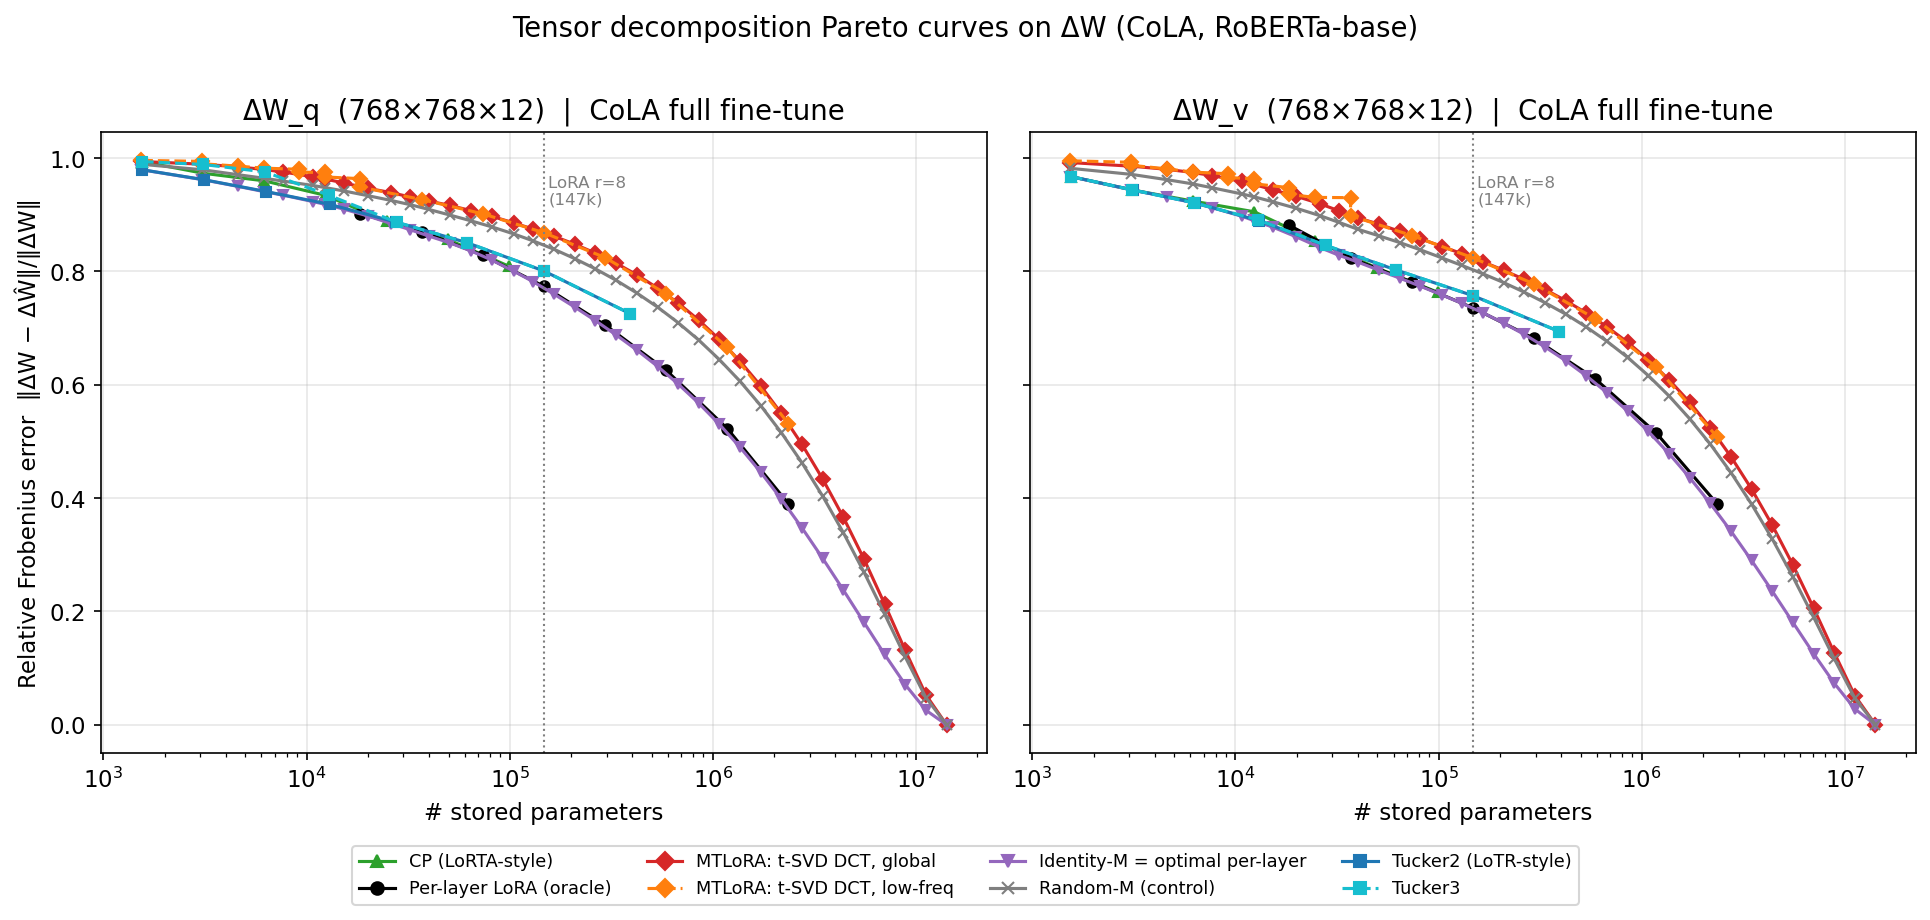
\includegraphics[width=\linewidth]{figures/pareto_curves.png}
\caption{Pareto error-vs-parameters curves for $\DeltaW_q$ (left) and $\DeltaW_v$ (right)
on CoLA. The identity-M t-SVD (purple triangles) dominates at tight error budgets.
DCT t-SVD (red diamonds) is not better than random-M (gray crosses), confirming
that $\DeltaW$ has no DCT-compressible depth structure.
Tucker-2 (LoTR, blue squares) and CP (green triangles) are competitive at loose error thresholds.}
\label{fig:pareto}
\end{figure}

% ─────────────────────────────────────────────────────────────────────────────
\section{Experiments}
\label{sec:experiments}

\subsection{Setup}
\label{sec:exp_setup}

We evaluate $\star_M$-LoRA on four GLUE \citep{wang2018glue} tasks using RoBERTa-base
\citep{liu2019roberta} as the backbone:
CoLA (Matthews Correlation Coefficient, MCC),
MRPC (paraphrase detection, accuracy),
RTE (textual entailment, accuracy), and
SST-2 (sentiment classification, accuracy).
All pretrained parameters are frozen; only the $\star_M$-LoRA adapter parameters and the
classification head are trained.
We use AdamW \citep{loshchilov2019adamw} with linear warmup over 6\% of steps
and gradient clipping at 1.0.
Unless noted, adapters are applied to query and value projections ($Q$, $V$),
rank $r=8$, $\alpha=4$, following LoRA and LoTR conventions.
Additional LoTR runs with $\alpha=1$ exist but are excluded from all tables.
The parameter-matched LoTR baseline uses rank 64 and $\alpha=32$, which keeps the scaling $\alpha/r=0.5$ of the
rank-8 runs.
With $M=I$ and $p=L=12$ the adapter is exactly one independent rank-8 pair $(A_\ell, B_\ell)$ per layer
(we verified $\Delta W_\ell = A_\ell B_\ell$ numerically), that is, per-layer LoRA, except that the output-side factor $\hat A$ is initialised
$\mathcal{N}(0,1)$ and the input-side factor $\hat B$ to zero, whereas standard LoRA \citep{hu2022lora} draws the input-side factor from a
Kaiming-uniform distribution ($U(\pm1/\sqrt{d_\mathrm{in}})$) and sets the output-side factor to zero.
We call the $\mathcal{N}(0,1)$ variant ``Identity'' and, because the initialisation turned out to matter, also run $M=I$, $p=L$ with the standard
initialisation (``LoRA''), which is the proper standard-LoRA baseline.
The Sections on transforms, $p$, initialisation and Cayley below report the earlier $\mathcal{N}(0,1)$-initialised variants; Section~\ref{sec:matched} repeats
DCT, random and Cayley $M$ with the standard initialisation (and the same learning rate, epochs, $\alpha/r=0.5$ and seeds as the LoRA rows), which is
the like-for-like comparison with standard LoRA.
LoTR uses a Kaiming-uniform initialisation of its shared factors and zero cores.
All scores are validation scores at the \emph{final} epoch; we do not select the best epoch.
Std.\ is the sample standard deviation over seeds.
The CoLA ablations in Sections~\ref{sec:transform_comparison}--\ref{sec:init_comparison} use five seeds (0--4) for the
$p=12$ DCT, $p=12$ random, $p=4$, $W_0$-guided ($p=4$) and Identity rows, and three seeds (0--2) for
$p\in\{1,2,6\}$; the pruning experiment in Section~\ref{sec:pruning_exp} is a single run.
Seed-to-seed std.\ on CoLA is $\approx$0.02 MCC
(Identity: $0.513\pm0.020$ over five seeds, range 0.480--0.534), so with three to five seeds per row differences
below about 0.03 MCC should not be over-interpreted.

\subsection{Transform comparison}
\label{sec:transform_comparison}

Table~\ref{tab:transforms} compares three transform choices with equal parameters
($p = L = 12$, $r = 8$, $\alpha = 4$, 5 epochs).

\begin{table}[h]
\centering
\caption{$\star_M$-LoRA with different transforms on CoLA (final-epoch val MCC, 5 epochs, rank=8, all 12 faces),
mean$\pm$std over seeds ($n$ in brackets).
All four variants have the same trainable parameter count (887,042 total, of which 294,912
are adapter parameters across $Q$+$V$).
All four rows use seeds 0--4 (on seeds 0--2 alone the rows are $0.541\pm0.016$ for DCT, $0.545\pm0.025$ for random and
$0.521\pm0.011$ for Identity).
Rank ordering of DCT and random is not established; see text.
The first three rows use the $\mathcal{N}(0,1)$ initialisation; ``Standard LoRA'' uses the Kaiming-uniform initialisation of Hu et al.}
\label{tab:transforms}
\begin{tabular}{lccc}
\toprule
Method & Adapter params & Total trainable & Val MCC (ep 5) \\
\midrule
$\star_M$-LoRA DCT         & 294,912 & 887,042 & 0.538$\pm$0.015 (5) \\
$\star_M$-LoRA Random-$M$  & 294,912 & 887,042 & 0.549$\pm$0.021 (5) \\
$\star_M$-LoRA Identity    & 294,912 & 887,042 & 0.513$\pm$0.020 (5) \\
Standard LoRA ($M=I$, usual init.) & 294,912 & 887,042 & 0.552$\pm$0.016 (5) \\
\midrule
LoRA $r=8$ (per-layer)$^\dagger$ & 147,456 & 295,680 & 0.515 \\
LoTR $r=32$$^\dagger$            &  74,496 &  76,032 & 0.613 \\
\bottomrule
\end{tabular}
{\small $^\dagger$Numbers from \citet{bershatsky2024lotr} on RoBERTa-base, 20 epochs; not directly comparable
due to different epoch count and learning rate.}
\end{table}

\noindent
DCT and a random orthogonal $M$ are indistinguishable ($0.538$ vs.\ $0.549$, Welch $p=0.35$; the random row is nominally higher),
so a fixed DCT has no advantage over an arbitrary orthogonal depth mixing.
That agrees with the absence of low-frequency depth structure in $\DeltaW$ (Section~\ref{sec:benchmark}).
Both are higher than Identity on the same five seeds, by $2.5$ points (DCT; Welch $p=0.055$, paired $p=0.055$) and $3.7$ points
(random; Welch $p=0.021$, paired $p=0.056$).
Pooling DCT and random against Identity gives $+3.1$ points ($p=0.020$).
With two comparisons the Bonferroni threshold is $0.025$, which the random-vs-Identity difference meets only barely and the DCT one does not,
and the pooled test was chosen after seeing the data, so we read the result as suggestive evidence that mixing layers through \emph{some}
orthogonal $M$ helps slightly at $p=L=12$ and 5 epochs, not as an established effect.
All three rows above are 5-epoch runs, and Identity gains $3.4$ points from training twice as long, so we also ran DCT and random $M$
for 10 epochs on the same five seeds (Table~\ref{tab:mixing}).
\textbf{The 5-epoch advantage does not persist.}
At 10 epochs DCT ($0.553\pm0.018$) and random $M$ ($0.555\pm0.016$) are $0.5$ and $0.7$ points above Identity ($0.548\pm0.017$, six seeds)
with Welch $p=0.66$ and $0.50$ (paired on the five shared seeds, $p=0.71$ and $0.47$), that is, indistinguishable.
From 5 to 10 epochs DCT gains $+1.5$ and random $M$ $+0.6$ points, against $+3.4$ for Identity, so the 5-epoch gap is better described as
faster early convergence of the mixed variants than as a higher final score.
Standard LoRA (same $M=I$, usual initialisation) is a stronger reference than Identity: it scores $0.552\pm0.016$ at 5 epochs and $0.590\pm0.013$ at 10 epochs,
so DCT and random $M$ are not above it at 5 epochs ($-1.4$ and $-0.3$ points, $p=0.19$ and $0.84$) and are \emph{below} it at 10 epochs
($-3.7$ and $-3.5$ points, $p=0.007$ and $0.005$).
The 5-epoch advantage of mixing over Identity is therefore consistent with the mixed variants compensating for the poorer $\mathcal{N}(0,1)$ initialisation, not with a benefit of mixing;
Section~\ref{sec:matched} tests this directly by giving DCT and random $M$ the standard initialisation.
The same holds on the other tasks (Table~\ref{tab:mixing}): on MRPC DCT and random $M$ are $1.1$ and $0.2$ points \emph{below} Identity, and on RTE
$0.3$ and $2.9$ points below, none significant ($p\ge0.3$).
We therefore find no final-score benefit from mixing layers through DCT or a random orthogonal $M$ on any of the four tasks we tested it on;
the 5-epoch CoLA result should be read as an optimisation-speed effect.
This is consistent with the Cayley experiment (Section~\ref{sec:multitask}), where learning $M$ did not help either.
The earlier single notebook runs (DCT 0.519, random 0.529, identity 0.543) are superseded by this table.

\begin{table}[h]
\centering
\caption{Layer mixing at $p=L=12$ ($r=8$, $\alpha=4$) beyond the 5-epoch CoLA setting: final-epoch score, mean$\pm$std ($n$ in brackets).
CoLA (MCC) at 10 epochs uses seeds 0--4 for DCT and random and seeds 0--4 and 42 for Identity; MRPC (accuracy, 5 epochs) and RTE (accuracy, 10 epochs, lr $10^{-4}$) use seeds 0--2
(Identity RTE and LoRA CoLA/RTE: seeds 0--4; LoRA MRPC: seeds 0--2).
$p$-values are Welch tests against Identity, uncorrected; LoRA is standard LoRA ($M=I$, usual initialisation).}
\label{tab:mixing}
\small
\begin{tabular}{lccc}
\toprule
Method & CoLA, 10 ep & MRPC & RTE \\
\midrule
Identity   & 0.548$\pm$0.017 (6) & 0.880$\pm$0.013 (3) & 0.691$\pm$0.012 (5) \\
DCT        & 0.553$\pm$0.018 (5), $p=0.66$ & 0.869$\pm$0.012 (3), $p=0.36$ & 0.688$\pm$0.015 (3), $p=0.81$ \\
Random $M$ & 0.555$\pm$0.016 (5), $p=0.50$ & 0.877$\pm$0.006 (3), $p=0.79$ & 0.662$\pm$0.036 (3), $p=0.30$ \\
\midrule
LoRA       & \textbf{0.590$\pm$0.013} (5), $p=0.001$ & 0.859$\pm$0.019 (3), $p=0.21$ & 0.653$\pm$0.023 (5), $p=0.016$ \\
\bottomrule
\end{tabular}
\end{table}

\subsection{n\_faces ablation}
\label{sec:faces_ablation}

Table~\ref{tab:nfaces} ablates the number of kept faces $p$ with DCT transform
and $r=8$.

\begin{table}[h]
\centering
\caption{$\star_M$-LoRA $n_{\text{faces}}$ ablation on CoLA (DCT, rank=8, $\alpha=4$, 5 epochs, $Q$+$V$).
Final-epoch val MCC, mean$\pm$std over seeds ($n$ in brackets: seeds 0--4 for $p=4$ and $p=12$, seeds 0--2 for the others);
$p$-values are Welch tests against $p=12$ (five seeds), uncorrected.
``Adapter params'' counts only $\hat{\cA}, \hat{\cB}$; total includes the 592,130-parameter classifier head.}
\label{tab:nfaces}
\begin{tabular}{lccccc}
\toprule
$p$ & Adapter params & Total trainable & Val MCC & $\Delta$ vs $p{=}12$ & Welch $p$-value \\
\midrule
1  &  24,576 & 616,706 & 0.436$\pm$0.026 (3) & $-$0.102 & 0.011 \\
2  &  49,152 & 641,282 & 0.475$\pm$0.010 (3) & $-$0.063 & 0.001 \\
4  &  98,304 & 690,434 & 0.503$\pm$0.024 (5) & $-$0.035 & 0.029 \\
6  & 147,456 & 739,586 & 0.520$\pm$0.013 (3) & $-$0.018 & 0.14 \\
12 & 294,912 & 887,042 & 0.538$\pm$0.015 (5) & --- & --- \\
\bottomrule
\end{tabular}
\end{table}

\noindent
Mean MCC increases monotonically with $p$ (0.436, 0.475, 0.503, 0.520, 0.538).
The drops at $p=1$ and $p=2$ are large relative to seed noise ($p=0.011$ and $0.001$, and they survive a Bonferroni threshold of
$0.0125$ for four comparisons), so one or two transform-domain faces are insufficient for this task.
The $p=4$ drop ($-3.5$ points, five seeds) has $p=0.029$, which does not survive the correction, and the $p=6$ drop
($-1.8$ points, three seeds) is of the order of the seed spread and is not significant.
$p=6$ reaches $97\%$ of the $p=12$ score at half the adapter parameters (147,456 vs.\ 294,912), so it may be a reasonable
trade-off, but with these data we cannot say that it matches $p=12$; $p=6$ has only three seeds.
Each of these runs keeps $p$ faces of a DCT, so ``fewer faces'' also means a low-pass depth projection.
To separate the effect of $p$ from that of the DCT we ran Identity with only the first $p$ layers adapted (with $M=I$ face $f$ is layer $f$, so layers $\ge p$ carry no adapter).
These runs did not train: for $p=4$ and $p=6$ all three seeds stay at MCC $0.0$ at every epoch with training loss $\approx0.61$,
which is the entropy of the CoLA label distribution (constant prediction).
We checked that the adapter itself is correct (layers $<p$ receive an update and layers $\ge p$ none).
Because Identity at $p=12$ is also unstable at learning rates $\ge10^{-3}$ (Section~\ref{sec:multitask}), the most likely reading is that
Identity with $N(0,1)$-initialised $\hat A$ at $5\times10^{-4}$ is unstable when the adapters are concentrated in early layers, so these runs say nothing about the benefit of larger $p$.
We therefore repeated the $p=6$ control with the standard LoRA initialisation (five seeds, same learning rate and epochs; Section~\ref{sec:matched}).
These runs do train, but reach only $0.443\pm0.024$ MCC against $0.548\pm0.011$ for DCT with $p=6$ (difference $+10.4$ points, $p<0.001$).
Adapting only the first six layers is therefore clearly worse than keeping six DCT faces that span all twelve layers, so with the same parameter count
the DCT projection is not merely a layer-count effect. This is not evidence that depth mixing helps beyond standard LoRA, because rank-4 LoRA with the same size reaches $0.550\pm0.011$.

\subsection{W\texorpdfstring{$_0$}{0}-guided initialization vs.\ random}
\label{sec:init_comparison}

Table~\ref{tab:init} compares random $A$-initialization with tSVD-M initialization
from $W_0$, both with $p=4$ DCT faces, rank 8, $\alpha=4$.

\begin{table}[h]
\centering
\caption{Initialization ablation on CoLA (DCT, $p=4$, rank=8, 690,434 trainable params).
``Random'' initializes $\hat{A}_f \sim \mathcal{N}(0,1)$, $\hat{B}_f=0$.
``W$_0$-guided'' initializes $\hat{A}_f$ from the top-$r$ left M-singular vectors of $\hat{W}_{0,f}$,
$\hat{B}_f=0$.
Mean val MCC per epoch over seeds 0--4 (five seeds each).}
\label{tab:init}
\begin{tabular}{lccccc}
\toprule
Init (seeds 0--4) & ep 1 & ep 2 & ep 3 & ep 4 & ep 5 \\
\midrule
Random         & 0.444 & 0.449 & 0.474 & 0.501 & 0.503 \\
$W_0$-guided   & 0.401 & 0.482 & 0.502 & 0.528 & 0.518 \\
\bottomrule
\end{tabular}
\end{table}

\noindent
Over the five seeds, $W_0$-guided initialization starts lower (epoch-1 MCC 0.401 vs.\ 0.444, with large seed-to-seed variation:
$0.348$, $0.385$, $0.475$, $0.337$, $0.461$ against $0.472$, $0.502$, $0.453$, $0.359$, $0.434$)
and is ahead from epoch 2 to epoch 5 (by $+3.3$, $+2.9$, $+2.7$ and $+1.5$ points), but the final-epoch gap is within seed noise
($0.518\pm0.009$ vs.\ $0.503\pm0.024$; Welch $p=0.25$, paired $p=0.31$).
No epoch shows a significant paired difference (smallest $p=0.061$, at epoch 3, uncorrected over five epochs).
The W$_0$-guided runs are less variable at epoch 5 (std $0.009$ vs.\ $0.024$), but with five seeds we do not read that as established.
The earlier single-run gap (0.518 vs.\ 0.495) is therefore not confirmed; we claim neither a benefit nor a cost of the
$W_0$-guided initialisation on final accuracy, though it may speed up the middle epochs.
The epoch-1 deficit is consistent with, but does not demonstrate, a somewhat slower start as in \citet{bershatsky2024lotr}'s finding that the adapter must first
escape the pretrained subspace.
The mean cosine between $\DeltaW_q$ and $W_0^{(q)}$'s left singular subspaces
(measured post-hoc) is only 0.172, confirming that the final adapter is nearly
orthogonal to $W_0$ regardless of initialization.

\subsection{Dynamic rank pruning}
\label{sec:pruning_exp}

Table~\ref{tab:pruning} compares $\star_M$-LoRA with and without face-level pruning
($p=12$, DCT, rank 8, $\alpha=4$, threshold $\tau=0.1$).

\begin{table}[h]
\centering
\caption{Dynamic face pruning on CoLA ($p=12$, DCT, rank=8, $\alpha=4$, 887,042 trainable params).
Pruning zeroes faces with $\|\hat{B}_f\|_F < 0.1$ after each epoch.
No faces were pruned in either run (all 12 faces remained active throughout).
Single run per row (notebook run), so the 0.519 is one draw from a seed spread of $\approx$0.02.}
\label{tab:pruning}
\begin{tabular}{lcccccc}
\toprule
Config & ep 1 & ep 2 & ep 3 & ep 4 & ep 5 & Faces pruned \\
\midrule
No pruning     & 0.480 & 0.521 & 0.490 & 0.532 & 0.519 & 0 \\
Pruning ($\tau{=}0.1$) & 0.480 & 0.521 & 0.490 & 0.532 & 0.519 & 0 \\
\bottomrule
\end{tabular}
\end{table}

\noindent
Both configurations produce identical training trajectories because no face was
pruned: all 12 faces grew $\|\hat{B}_f\|_F \gg 0.1$ by the end of epoch 1.
This indicates that with a standard learning rate ($5 \times 10^{-4}$), all
transform-domain faces receive sufficient gradient signal to remain active.
Dynamic pruning is most effective when M is learnable (so low-energy faces have
genuinely low information content in the task basis), or when a much higher
threshold $\tau$ is used in conjunction with $W_0$-guided initialization.

\subsection{Learnable-$M$ ($\star_M$-LoRA-Cayley) on CoLA}
\label{sec:cayley_exp}

Table~\ref{tab:cayley} reports the per-epoch MCC of $\star_M$-LoRA-Cayley
($p=12$, rank=8, $\alpha=4$, freeze$_M$=2 epochs, $\eta_{AB}=5\times10^{-4}$,
$\eta_M=10^{-3}$, 10 epochs, $Q$+$V$).

\begin{table}[h]
\centering
\caption{$\star_M$-LoRA-Cayley on CoLA (val MCC per epoch, rank=8, $p=12$).
M is frozen for epochs 1--2 (warm-up), then jointly optimised.
``M\_rot'' is $\|M - I\|_F$ at epoch end.
Total trainable params: 592,130 (head) + 147,522 (Q adapter) + 147,522 (V adapter) = 887,174.}
\label{tab:cayley}
\begin{tabular}{ccccc}
\toprule
Epoch & Val MCC & Train loss & M\_rot & M frozen? \\
\midrule
1  & 0.293 & 0.562 & 0.000 & Yes \\
2  & 0.452 & 0.475 & 0.000 & Yes \\
3  & 0.444 & 0.430 & 0.303 & No \\
4  & 0.496 & 0.371 & 0.343 & No \\
5  & 0.515 & 0.332 & 0.421 & No \\
6  & 0.521 & 0.299 & 0.448 & No \\
7  & 0.497 & 0.259 & 0.453 & No \\
8  & 0.539 & 0.235 & 0.449 & No \\
9  & 0.539 & 0.201 & 0.456 & No \\
10 & \textbf{0.547} & 0.194 & 0.456 & No \\
\bottomrule
\end{tabular}
\end{table}

\noindent
The run in Table~\ref{tab:cayley} (seed 42) reaches MCC 0.547 at epoch 10.
Over six seeds (0, 1, 2, 3, 4, 42) $\star_M$-LoRA-Cayley reaches $0.540\pm0.013$ at epoch 10,
using only 132 additional Cayley parameters across the two adapter families (66 per family).
The M rotation grows from 0 at epoch 2 to $\|M-I\|_F = 0.43$--$0.59$ by epoch 10 across seeds
(0.456 for seed 42), confirming that the Cayley parameters actively learn a non-trivial depth
basis during fine-tuning.
Against $\star_M$-LoRA-Identity trained for the same 10 epochs and the same six seeds
($0.548\pm0.017$) the difference is $-0.8$ MCC points; it is negative for four of the six seeds
(range $-2.0$ to $+1.0$), and a paired $t$-test gives $p=0.17$.
The gap is therefore not statistically distinguishable from zero.
At 5 epochs, Cayley reaches $0.513\pm0.015$ and Identity $0.513\pm0.020$ over five seeds (difference $+0.06$ points,
$p=0.96$), with $\|M-I\|_F\approx0.2$ at that point.
Training Identity for 10 instead of 5 epochs improves it by $+$3.4 MCC points on the same five seeds
($0.513\to0.547$), so the 5-epoch CoLA ablations above are under-trained relative to the 10-epoch rows.
The dip at epoch 7 in the seed-42 run (0.497) and its recovery to 0.539--0.547 at epochs 8--10
suggests that M undergoes a brief reorganisation after escaping the identity basin.
Section~\ref{sec:multitask} compares Cayley with Identity at matched epochs.

\subsection{Initialisation-matched comparison with standard LoRA}
\label{sec:matched}

The comparisons above give DCT, random and Cayley $M$ the $\mathcal{N}(0,1)$ initialisation, which is 3.9--4.2 points worse than the standard LoRA initialisation for the
same $M=I$ adapter on CoLA.
To compare coupling with standard LoRA like for like, we reran DCT, random and Cayley $M$ ($p=12$, $r=8$, $\alpha=4$) with the standard initialisation
(input-side factor $U(\pm1/\sqrt{d_\mathrm{in}})$, output-side factor zero), using the same learning rate, epochs and seeds as the LoRA rows of Table~\ref{tab:glue}
(CoLA: 5 and 10 epochs, seeds 0--4; MRPC and SST-2: 5 epochs, seeds 0--2; RTE: 10 epochs, lr $10^{-4}$, seeds 0--4).
Table~\ref{tab:matched} reports the difference to standard LoRA with a 95\% Welch confidence interval.

\begin{table}[h]
\centering
\caption{Coupling vs.\ standard LoRA at matched initialisation, learning rate, epochs and seeds. Entries are the mean score of each method (final epoch),
with the difference to standard LoRA and its 95\% Welch confidence interval in points (MCC $\times100$ for CoLA, accuracy $\times100$ otherwise) below.
$n$ as in Table~\ref{tab:glue}. All differences are consistent with zero.}
\label{tab:matched}
\small
\setlength{\tabcolsep}{3pt}
\resizebox{\linewidth}{!}{%
\begin{tabular}{lccccc}
\toprule
Method (LoRA init.) & CoLA 5 ep & CoLA 10 ep & MRPC & RTE & SST-2 \\
\midrule
Standard LoRA ($M=I$) & 0.552 & 0.590 & 0.859 & 0.653 & 0.938 \\
\midrule
DCT, $p=12$ & 0.562 & 0.586 & 0.868 & 0.630 & 0.938 \\
\quad vs.\ LoRA & $+1.0$ [$-1.1$, $+3.1$] & $-0.4$ [$-2.3$, $+1.4$] & $+0.8$ [$-3.2$, $+4.8$] & $-2.3$ [$-6.0$, $+1.4$] & $+0.0$ [$-0.9$, $+0.9$] \\
Random $M$, $p=12$ & 0.564 & 0.585 & 0.862 & 0.642 & 0.943 \\
\quad vs.\ LoRA & $+1.2$ [$-0.9$, $+3.3$] & $-0.5$ [$-2.4$, $+1.5$] & $+0.2$ [$-4.3$, $+4.8$] & $-1.1$ [$-4.9$, $+2.7$] & $+0.5$ [$-0.4$, $+1.3$] \\
Cayley $M$, $p=12$ & 0.555 & 0.588 & 0.862 & 0.654 & 0.937 \\
\quad vs.\ LoRA & $+0.4$ [$-1.8$, $+2.5$] & $-0.2$ [$-2.4$, $+2.1$] & $+0.2$ [$-3.6$, $+4.1$] & $+0.1$ [$-3.2$, $+3.5$] & $-0.1$ [$-1.0$, $+0.7$] \\
\bottomrule
\end{tabular}%
}
\end{table}

\noindent
\textbf{With matched initialisation, no coupled variant differs from standard LoRA.}
On CoLA the three variants are $+1.0$, $+1.2$ and $+0.4$ points above LoRA at 5 epochs and $-0.4$, $-0.5$ and $-0.2$ points at 10 epochs, all with Welch $p\ge0.23$;
the sign changes between 5 and 10 epochs and the intervals include zero.
On RTE the DCT and random variants are nominally lower ($-2.3$ and $-1.1$ points) and on MRPC and SST-2 nominally higher by at most $0.8$ points, none significant.
The initialisation matters for coupling as much as for LoRA: DCT with the standard initialisation is $2.4$ points better at 5 epochs ($p=0.022$) and $3.3$ points better at 10 epochs ($p=0.012$) than DCT with $\mathcal{N}(0,1)$.
Together with Section~\ref{sec:transform_comparison}, this supports reading the earlier 5-epoch advantage of DCT and random $M$ over Identity as an initialisation effect.
Per-epoch validation curves of LoRA, DCT and random $M$ on CoLA are close at every epoch (epoch 1: $0.449$, $0.456$, $0.469$; epoch 5: $0.552$, $0.562$, $0.564$), so there is no clear early-convergence advantage either.

\textbf{Power.}
With five seeds and a standard deviation of about $0.015$ MCC, a two-sided Welch test at $\alpha=0.05$ has 80\% power for a true difference of about $3.0$ points on CoLA; for RTE (five seeds, std $\approx0.025$) it is about $5$ points, for MRPC (three seeds) about $4$ points and for SST-2 (three seeds) about $0.9$ points.
The confidence intervals in Table~\ref{tab:matched} are consistent with differences of up to about $\pm2$ to $3$ points on CoLA and $\pm4$ to $6$ points on MRPC and RTE, so we can exclude large effects but not
small ones (a benefit of one or two MCC points on CoLA, for example, cannot be ruled out).

\textbf{Equal-budget test.}
The setting in which a cross-layer method has the best chance of an advantage is at a smaller adapter size than per-layer LoRA.
We therefore compared DCT with $p=6$ faces ($147{,}456$ adapter parameters, standard initialisation) with standard LoRA of rank 4, which has the same number of adapter parameters,
and with $M=I$ adapting only the first six layers (CoLA, 5 epochs, five seeds each).
DCT $p=6$ scores $0.548\pm0.011$, rank-4 LoRA $0.550\pm0.011$ ($-0.2$ points, 95\% interval $[-1.8,+1.4]$, $p=0.77$), and $M=I$ on six layers only $0.443\pm0.024$ ($+10.4$ points for DCT, $p<0.001$, higher on all five seeds).
Rank-4 LoRA is within $0.2$ points of rank-8 LoRA ($0.552\pm0.016$), so on CoLA at this scale halving the adapter size costs nothing.
Two things follow.
First, mixing through $M$ is clearly better than dropping layers: with six faces the DCT adapter reaches layers that $M=I$ with six faces cannot reach.
Second, this advantage is not specific to mixing, since an equally sized \emph{uniform} low-rank adapter (rank 4 on all twelve layers) does just as well.
So the earlier finding that accuracy rises with the number of faces $p$ (Section~\ref{sec:faces_ablation}) is not evidence for a depth-mixing benefit beyond the adapter's total capacity.
The Identity control also resolves the question left open there: with the standard initialisation the six-layer Identity adapter does train (it did not with $\mathcal{N}(0,1)$), and it is much worse than DCT with six faces.

\textbf{Learning-rate controls.}
Standard LoRA is not at its best learning rate at $5\times10^{-4}$ on CoLA or at $10^{-4}$ on RTE, and neither is DCT, so we ran both over a wider grid (three seeds per cell, 5 epochs for CoLA, 10 for RTE; Table~\ref{tab:matched_lr}).
On CoLA both improve up to $10^{-3}$--$2\times10^{-3}$ (LoRA $0.591\pm0.010$ at $10^{-3}$ and $0.593\pm0.012$ at $2\times10^{-3}$; DCT $0.590\pm0.020$ at $10^{-3}$) and the two are within $0.1$--$1.4$ points of each other at every learning rate.
On RTE both reach about $0.74$ at $10^{-3}$ (LoRA $0.740\pm0.016$, DCT $0.746\pm0.002$; difference $+0.6$ points, $p=0.58$), a $4.9$-point improvement for LoRA over Identity at its own best learning rate ($0.691$, $p=0.014$).
The headline RTE comparison at $10^{-4}$ therefore under-trained both LoRA-initialised variants, and its apparent $-2.3$ points for DCT does not persist at a larger learning rate.
Comparing the best learning rate of each method on CoLA, LoRA ($0.591\pm0.010$) is $1.7$ points above rank-64 LoTR at its best ($0.574\pm0.008$; Welch $p=0.09$, paired over seeds $p=0.03$, three seeds); on RTE LoRA at $10^{-3}$ is $2.3$ points above LoTR at its best ($0.717\pm0.018$, $p=0.17$).
None of these tuned comparisons is significant under a Bonferroni correction, and the grids and best values are selected on validation scores.

\begin{table}[h]
\centering
\caption{Learning-rate controls with the standard initialisation (final-epoch score, mean$\pm$std, $n=3$ except where noted: LoRA and DCT at $5\times10^{-4}$ on CoLA and at $10^{-4}$ on RTE, $n=5$).
Bold marks the best value of each column on this grid (selected on the reported scores, hence optimistic).
Identity is the $\mathcal{N}(0,1)$-initialised $M=I$ adapter; ``---'' = not run.}
\label{tab:matched_lr}
\small
\setlength{\tabcolsep}{3pt}
\resizebox{\linewidth}{!}{%
\begin{tabular}{lccccccc}
\toprule
 & \multicolumn{4}{c}{CoLA (MCC, 5 ep)} & \multicolumn{3}{c}{RTE (acc., 10 ep)} \\
\cmidrule(lr){2-5}\cmidrule(lr){6-8}
Learning rate & LoRA & DCT & LoTR-64 & Identity & LoRA & DCT & Identity \\
\midrule
$10^{-4}$        & --- & --- & --- & 0.466$\pm$0.028 & 0.653$\pm$0.023 & 0.630$\pm$0.027 & \textbf{0.691$\pm$0.012} \\
$2\times10^{-4}$ & 0.526$\pm$0.026 & 0.523$\pm$0.016 & 0.515$\pm$0.004 & 0.504$\pm$0.019 & --- & --- & --- \\
$3\times10^{-4}$ & --- & --- & --- & --- & 0.700$\pm$0.007 & 0.705$\pm$0.008 & 0.681$\pm$0.034 \\
$5\times10^{-4}$ & 0.552$\pm$0.016 & 0.562$\pm$0.011 & 0.557$\pm$0.020 & \textbf{0.513$\pm$0.020} & --- & --- & --- \\
$10^{-3}$        & 0.591$\pm$0.010 & \textbf{0.590$\pm$0.020} & \textbf{0.574$\pm$0.008} & 0.000$\pm$0.000 & \textbf{0.740$\pm$0.016} & \textbf{0.746$\pm$0.002} & 0.509$\pm$0.031 \\
$2\times10^{-3}$ & \textbf{0.593$\pm$0.012} & 0.580$\pm$0.015 & 0.376$\pm$0.326 & 0.000$\pm$0.000 & --- & --- & --- \\
\bottomrule
\end{tabular}%
}
\end{table}

\textbf{What the step-size hypothesis does and does not explain.}
The $\mathcal{N}(0,1)$ Identity adapter cannot be repaired simply by lowering the learning rate.
Its output-side factor is about fifty times larger than the standard one, so one Adam step at the same learning rate changes $\Delta W$ about fifty times more (a first-step calculation, not a measurement during training).
Lowering the learning rate to $10^{-4}$, $3\times10^{-5}$ and $10^{-5}$ does not help on CoLA: Identity scores $0.466\pm0.028$, $0.392\pm0.004$ and $0.000$ (no learning),
all below its $0.513\pm0.020$ at $5\times10^{-4}$, and it fails above $10^{-3}$.
So its stable range is narrow on both sides and its best value remains $4$--$8$ points below standard LoRA, which means that the step-size argument alone does not explain the gap
and we do not claim a mechanism for the initialisation effect.

\subsection{Small adapter budgets}
\label{sec:budget}

The matched comparison above uses a generous adapter (rank 8, 295K adapter parameters), where per-layer LoRA already has ample capacity.
The structural argument for a cross-layer adapter is strongest at a small budget.
DCT with $p$ faces and rank $r$ has $p\,r$ ``rank-units'' (adapter parameters $=p\,r\,(d_\mathrm{out}+d_\mathrm{in})$ per projection), and each layer's $\Delta W_\ell$ can have rank up to $p\,r$;
per-layer LoRA with the same parameters has rank $p\,r/L$ in each layer, for example rank 1 against rank 6 with $p=2$ at 12 rank-units.
We therefore compared, at three budgets (12, 24 and 48 rank-units, i.e.\ LoRA rank 1, 2 and 4, with 37K, 74K and 147K adapter parameters), standard LoRA with DCT at $p=2$ and $p=6$,
random $M$ at $p=2$, and Identity on the first two layers only as a control, all with the standard initialisation, $\alpha/r=0.5$, learning rate $10^{-3}$ and five seeds
(CoLA 5 epochs, RTE 10 epochs).
Within a budget every configuration has exactly the same number of adapter parameters.

\begin{table}[h]
\centering
\caption{Equal-parameter comparison at small adapter budgets (RoBERTa-base, standard initialisation, lr $10^{-3}$, five seeds, final epoch).
Mean $\pm$ s.d.\ of CoLA MCC and RTE accuracy, with the difference to standard LoRA of the same budget in points in parentheses.}
\label{tab:budget}
\small
\setlength{\tabcolsep}{4pt}
\resizebox{\linewidth}{!}{%
\begin{tabular}{lcc}
\toprule
Method & CoLA (MCC) & RTE (acc.) \\
\midrule
\multicolumn{3}{l}{\emph{Budget 12 rank-units (36,864 adapter parameters; LoRA rank 1)}} \\
Standard LoRA (all 12 layers), $r=1$ & 0.541$\pm$0.007 & 0.712$\pm$0.009 \\
DCT, $p=2$, $r=6$ & 0.521$\pm$0.009 ($-$1.9) & 0.687$\pm$0.015 ($-$2.5) \\
DCT, $p=6$, $r=2$ & 0.532$\pm$0.014 ($-$0.9) & 0.691$\pm$0.011 ($-$2.1) \\
Random $M$, $p=2$, $r=6$ & 0.510$\pm$0.026 ($-$3.0) & 0.696$\pm$0.014 ($-$1.6) \\
Identity, first 2 layers only, $r=6$ & 0.301$\pm$0.024 ($-$24.0) & 0.591$\pm$0.009 ($-$12.1) \\
\midrule
\multicolumn{3}{l}{\emph{Budget 24 rank-units (73,728 adapter parameters; LoRA rank 2)}} \\
Standard LoRA (all 12 layers), $r=2$ & 0.559$\pm$0.011 & 0.713$\pm$0.008 \\
DCT, $p=2$, $r=12$ & 0.539$\pm$0.014 ($-$2.1) & 0.705$\pm$0.012 ($-$0.7) \\
DCT, $p=6$, $r=4$ & 0.555$\pm$0.009 ($-$0.4) & 0.723$\pm$0.010 ($+$1.1) \\
Random $M$, $p=2$, $r=12$ & 0.542$\pm$0.004 ($-$1.7) & 0.706$\pm$0.014 ($-$0.6) \\
Identity, first 2 layers only, $r=12$ & 0.269$\pm$0.035 ($-$29.0) & 0.620$\pm$0.015 ($-$9.2) \\
\midrule
\multicolumn{3}{l}{\emph{Budget 48 rank-units (147,456 adapter parameters; LoRA rank 4)}} \\
Standard LoRA (all 12 layers), $r=4$ & 0.568$\pm$0.012 & 0.731$\pm$0.023 \\
DCT, $p=2$, $r=24$ & 0.439$\pm$0.246 ($-$12.9) & 0.721$\pm$0.019 ($-$1.0) \\
DCT, $p=6$, $r=8$ & 0.559$\pm$0.011 ($-$0.9) & 0.729$\pm$0.021 ($-$0.2) \\
Random $M$, $p=2$, $r=24$ & 0.540$\pm$0.011 ($-$2.9) & 0.720$\pm$0.012 ($-$1.2) \\
Identity, first 2 layers only, $r=24$ & 0.309$\pm$0.058 ($-$25.9) & 0.589$\pm$0.042 ($-$14.2) \\
\bottomrule
\end{tabular}%
}
\end{table}

Coupling does not help at any budget (Table~\ref{tab:budget}).
Of the 18 comparisons of DCT or random $M$ with LoRA of the same size, 17 point estimates are below LoRA and one is above it (DCT $p=6$ on RTE at 24 units, $+1.1$ points, $p=0.11$).
On CoLA the DCT and random configurations with $p=2$ are $1.7$--$3.0$ points below LoRA (Welch $p$ between $0.005$ and $0.057$; the exception is DCT $p=2$ at 48 units, which includes the failed run described below), and on RTE the largest gaps are $2.5$ points (DCT $p=2$, $p=0.018$) and $2.1$ points (DCT $p=6$, $p=0.012$) at the smallest budget.
None of these survives a Holm correction over the 18 comparisons (smallest adjusted $p=0.084$), so we describe them as weak evidence that coupling is slightly worse rather than as a demonstrated loss.
The comparisons share the LoRA reference within a budget and are not independent.
The benefit predicted by the rank argument, a higher per-layer rank at the same size, does not appear.
DCT with $p=2$ keeps only the two lowest depth frequencies, so $\Delta W_\ell$ varies smoothly with $\ell$; we did not test whether this restriction, rather than the rank, explains the result.

The Identity control is a placement test, not a variant of LoRA: with $M=I$ face $f$ is layer $f$, so keeping $p=2$ faces places two large adapters in layers 0 and 1 and leaves the other ten layers without any adapter, whereas LoRA of the same size places a small adapter in every layer.
Concentrating the budget in two layers is far worse than spreading it, either with DCT or with LoRA ($-24$ to $-29$ points on CoLA and $-9$ to $-14$ on RTE), so the DCT projection does spread a small budget over all layers, but it does not beat spreading it by lowering the rank.
A possible reason, which we did not test, is that with $p=2$ the DCT update of every layer is a fixed scalar combination of two shared matrices (a constant and a linear ramp over depth), so the layers receive nearly the same update, while LoRA gives each layer its own direction and fine-tuning updates differ by layer; the DCT coefficients are also about $1/\sqrt{L}\approx0.29$ in size, which lowers the effective step, and we did not separate this from the loss of layer-specific freedom.
One DCT $p=2$, $r=24$ run on CoLA (seed 4) never left constant prediction (MCC $0$, training loss $0.61$); the other four seeds reach $0.549\pm0.018$, which is $2.0$ points below rank-4 LoRA ($p=0.12$).
The table reports all five seeds, which is why that cell has a large standard deviation ($0.439\pm0.246$); LoRA and the other configurations had no such failure.
At the smallest budget, LoRA rank 1 improves with the learning rate ($0.517$, $0.541$, $0.575$ at $5\times10^{-4}$, $10^{-3}$, $2\times10^{-3}$; three seeds at the outer values) and DCT $p=2$ does too ($0.496$, $0.521$, $0.546$), so the ordering is the same at every rate and the gap, $2$--$3$ points, is not a learning-rate artefact.
LoRA was still improving at $2\times10^{-3}$, the upper end of the grid, so the best rates for both methods are not established.

\subsection{Learned $M$ in the small-budget and deeper-model regimes}
\label{sec:cayley_budget}

A learned $M$ could in principle find a depth basis that a fixed DCT or random $M$ misses, so we repeated the $p=2$ small-budget comparison with the Cayley parametrisation (Section~\ref{sec:learnable_M}).
We trained it with the same script, schedule, learning rate, epochs and seeds as the fixed-$M$ runs of Section~\ref{sec:budget}, with $S$ frozen for the first two epochs, in three variants:
$M$ started at the DCT matrix with $\eta_M=10^{-3}$ or $10^{-2}$, and $M$ started at the identity with $\eta_M=10^{-2}$.
A DCT start with frozen $S$ reproduces the fixed-DCT run, so each DCT-start run is paired with a fixed-DCT run of the same seed.
(In the DCT-start runs $M$ moved little: the Frobenius distance from the DCT matrix at the end of training was $0.19$ on CoLA and $0.36$ on RTE with $\eta_M=10^{-3}$ and $0.80$ and $1.3$ with $\eta_M=10^{-2}$, compared with a maximum of about $6.9$ for $L=12$.
From the identity it reached $2.8$ and $3.3$.)

\begin{table}[h]
\centering
\caption{Learned (Cayley) $M$ against fixed $M$ and standard LoRA at the same number of adapter parameters (RoBERTa-base, five seeds, lr $10^{-3}$, final epoch).
Mean $\pm$ s.d.\ and the difference to standard LoRA of the same budget in points in parentheses.}
\label{tab:cayley_budget}
\small
\setlength{\tabcolsep}{4pt}
\resizebox{\linewidth}{!}{%
\begin{tabular}{lcc}
\toprule
Method & CoLA (MCC) & RTE (acc.) \\
\midrule
\multicolumn{3}{l}{\emph{Budget 12 rank-units (LoRA rank 1)}} \\
Standard LoRA & 0.541$\pm$0.007 & 0.712$\pm$0.009 \\
DCT, $p=2$ (fixed) & 0.521$\pm$0.009 ($-$1.9) & 0.687$\pm$0.015 ($-$2.5) \\
Cayley, DCT start, $\eta_M=10^{-3}$ & 0.529$\pm$0.018 ($-$1.2) & 0.691$\pm$0.026 ($-$2.1) \\
Cayley, DCT start, $\eta_M=10^{-2}$ & 0.524$\pm$0.020 ($-$1.7) & 0.693$\pm$0.009 ($-$1.9) \\
Cayley, identity start, $\eta_M=10^{-2}$ & 0.458$\pm$0.011 ($-$8.2) & 0.685$\pm$0.010 ($-$2.7) \\
Identity, $p=2$ (fixed) & 0.301$\pm$0.024 ($-$24.0) & 0.591$\pm$0.009 ($-$12.1) \\
\midrule
\multicolumn{3}{l}{\emph{Budget 24 rank-units (LoRA rank 2)}} \\
Standard LoRA & 0.559$\pm$0.011 & 0.713$\pm$0.008 \\
DCT, $p=2$ (fixed) & 0.539$\pm$0.014 ($-$2.1) & 0.705$\pm$0.012 ($-$0.7) \\
Cayley, DCT start, $\eta_M=10^{-3}$ & 0.531$\pm$0.013 ($-$2.8) & 0.712$\pm$0.014 ($-$0.1) \\
Cayley, DCT start, $\eta_M=10^{-2}$ & 0.536$\pm$0.014 ($-$2.3) & 0.707$\pm$0.017 ($-$0.6) \\
Cayley, identity start, $\eta_M=10^{-2}$ & 0.462$\pm$0.024 ($-$9.7) & 0.621$\pm$0.069 ($-$9.2) \\
Identity, $p=2$ (fixed) & 0.269$\pm$0.035 ($-$29.0) & 0.620$\pm$0.015 ($-$9.2) \\
\midrule
\multicolumn{3}{l}{\emph{Budget 48 rank-units (LoRA rank 4)}} \\
Standard LoRA & 0.568$\pm$0.012 & 0.731$\pm$0.023 \\
DCT, $p=2$ (fixed) & 0.439$\pm$0.246 ($-$12.9) & 0.721$\pm$0.019 ($-$1.0) \\
Cayley, DCT start, $\eta_M=10^{-3}$ & 0.552$\pm$0.015 ($-$1.6) & 0.728$\pm$0.007 ($-$0.4) \\
Cayley, DCT start, $\eta_M=10^{-2}$ & 0.555$\pm$0.012 ($-$1.3) & 0.723$\pm$0.016 ($-$0.8) \\
Cayley, identity start, $\eta_M=10^{-2}$ & 0.489$\pm$0.017 ($-$8.0) & 0.687$\pm$0.032 ($-$4.5) \\
Identity, $p=2$ (fixed) & 0.309$\pm$0.058 ($-$25.9) & 0.589$\pm$0.042 ($-$14.2) \\
\bottomrule
\end{tabular}%
}
\end{table}

Learning $M$ does not help (Table~\ref{tab:cayley_budget}).
All 12 comparisons of the two DCT-start variants with standard LoRA are below LoRA (by $0.1$ to $2.8$ points); the largest gaps are $2.8$ points on CoLA (24 units, $p=0.007$) and $2.1$ points on RTE (12 units, $p=0.15$), and after a Holm correction over the 18 Cayley comparisons none of the DCT-start differences is significant (smallest adjusted $p=0.094$).
Against the fixed-DCT runs of the same seed the learned $M$ makes essentially no difference: the paired differences are $-0.7$ to $+0.8$ points on CoLA and $+0.1$ to $+0.7$ points on RTE at every budget and learning rate (paired $p\geq0.16$ in every cell; pooled mean $+0.3\pm1.8$ points over 29 pairs, $p=0.37$ for $\eta_M=10^{-3}$ and $+0.3\pm1.5$, $p=0.35$ for $\eta_M=10^{-2}$).
A pooled gain of 0.3 points is far smaller than the seed standard deviation and than the $1$--$3$ point gap to LoRA that learning $M$ would have to close.
Two of the 30 DCT-start runs followed a different first epoch from their fixed-DCT partner although $S$ was still frozen (the two $M$ differ by about $10^{-6}$ from the float32 Cayley reconstruction): in one (CoLA, 48 units, seed 4) the fixed-DCT run stayed at constant prediction while the Cayley run trained (MCC $0.56$), in the other (24 units, seed 2) the fixed run left constant prediction one epoch later.
The first pair is excluded from the paired comparison, and we do not claim that the learned $M$ made training more stable; the difference comes from numerical noise before $M$ was unfrozen.
Starting from the identity, the learned $M$ is far better than Identity on the first two layers ($+9$ to $+19$ points on CoLA and RTE, except $+0.1$ on RTE at 24 units, where one of the five seeds scored only $0.54$), but still $8$--$10$ points below LoRA on CoLA and $2.7$--$9.2$ points below on RTE (Holm-adjusted $p<0.05$ on CoLA at all three budgets and on RTE at 12 units).
So $M$ can learn to spread a small budget over the layers that a first-two-layers $M=I$ cannot reach, but on CoLA it ended $6$--$8$ points below the fixed DCT (paired $p\le0.002$ at every budget) and on RTE $0.2$--$8.5$ points below (not significant), so it did not find a basis as good as the DCT, let alone LoRA, within the training budget.

\subsection{More training data}
\label{sec:moredata}

The GLUE tasks above have 2.5k--67k training examples; with more data a cross-layer adapter has more signal from which to learn a shared depth basis.
We repeated the comparison on QNLI (105k examples) and MNLI (393k examples; matched validation set), RoBERTa-base, 3 epochs, learning rate $5\times10^{-4}$, standard initialisation, three seeds,
at three adapter sizes (Table~\ref{tab:moredata}).
The small-budget pairs have the same number of adapter parameters; the 96-unit pair is the headline configuration (DCT $p=12$ against LoRA, rank 8).

\begin{table}[h]
\centering
\caption{Coupling vs.\ LoRA with more training data (RoBERTa-base, three seeds, final epoch, standard initialisation, lr $5\times10^{-4}$).
Mean $\pm$ s.d.\ and the difference (points) to LoRA of the same size with its 95\% Welch interval.}
\label{tab:moredata}
\small
\setlength{\tabcolsep}{4pt}
\resizebox{\linewidth}{!}{%
\begin{tabular}{lccc}
\toprule
Comparison & LoRA & DCT & DCT $-$ LoRA [95\% CI] \\
\midrule
\multicolumn{4}{l}{\emph{MNLI-m (acc.)}} \\
12 units (LoRA $r=1$) vs.\ DCT $p=2$, $r=6$ & 0.850$\pm$0.001 & 0.838$\pm$0.001 & $-$1.1 [$-$1.4, $-$0.8] \\
24 units (LoRA $r=2$) vs.\ DCT $p=2$, $r=12$ & 0.855$\pm$0.000 & 0.844$\pm$0.001 & $-$1.0 [$-$1.3, $-$0.8] \\
96 units (LoRA $r=8$) vs.\ DCT $p=12$, $r=8$ & 0.864$\pm$0.001 & 0.863$\pm$0.001 & $-$0.2 [$-$0.5, $+$0.1] \\
\midrule
\multicolumn{4}{l}{\emph{QNLI (acc.)}} \\
12 units (LoRA $r=1$) vs.\ DCT $p=2$, $r=6$ & 0.904$\pm$0.003 & 0.900$\pm$0.003 & $-$0.4 [$-$1.0, $+$0.2] \\
24 units (LoRA $r=2$) vs.\ DCT $p=2$, $r=12$ & 0.910$\pm$0.001 & 0.903$\pm$0.002 & $-$0.6 [$-$1.1, $-$0.2] \\
96 units (LoRA $r=8$) vs.\ DCT $p=12$, $r=8$ & 0.919$\pm$0.001 & 0.917$\pm$0.003 & $-$0.1 [$-$0.8, $+$0.5] \\
\bottomrule
\end{tabular}%
}
\end{table}

More data does not help the coupled adapter; the sign of every difference is negative (Table~\ref{tab:moredata}).
On MNLI, DCT $p=2$ is $1.1$ and $1.0$ points below LoRA of the same size at 12 and 24 units (Welch $p<0.001$ and $p=0.003$, Holm-adjusted $p=0.017$ and $0.13$ over all 45 comparisons in this paper's small-budget, data and deeper-model experiments);
at the 96-unit headline size the difference is $-0.2$ points (interval $[-0.5,+0.1]$).
On QNLI the differences are $-0.1$ to $-0.6$ points and each interval is consistent with 0 or with a small loss.
The MNLI result at the smallest budgets is the only comparison in this paper that survives a multiplicity correction, and the gap is about one point; with three seeds and one learning rate we do not claim more than that.

\subsection{Deeper models}
\label{sec:deeper}

A twelve-layer encoder may simply be too shallow for depth-sharing to pay off.
We ran the same adapters on decoder-only models of depth $L=28$ (Qwen2.5-1.5B and Qwen2.5-7B, query and value projections, frozen bfloat16 base, float32 adapters and classification head, 3 epochs, three seeds, standard initialisation, $\alpha/r=0.5$).
We used Qwen2.5 because Llama-3-8B is gated; the depth ($L=28$) is close to Llama-3-8B's 32.
At 28 rank-units LoRA has rank 1 in each layer; the coupled adapters have the same number of parameters (139K for 1.5B, 323K for 7B).
At 224 units the comparison is rank-8 LoRA against $p=28$, $r=8$ (1.09M and 2.53M adapter parameters).
Learning rate is $2\times10^{-4}$ for 1.5B and $10^{-4}$ for 7B (Table~\ref{tab:llm}).

\begin{table}[h]
\centering
\caption{Coupling vs.\ LoRA in deeper models ($L=28$, three seeds, final epoch). Mean $\pm$ s.d.\ and the difference (points) to LoRA of the same adapter size with its 95\% Welch interval.}
\label{tab:llm}
\small
\setlength{\tabcolsep}{3pt}
\resizebox{\linewidth}{!}{%
\begin{tabular}{lccc}
\toprule
Comparison & LoRA & Coupled & Coupled $-$ LoRA [95\% CI] \\
\midrule
\multicolumn{4}{l}{\emph{Qwen2.5-1.5B ($L=28$)}} \\
CoLA (MCC), 28 units: LoRA $r=1$ vs.\ DCT $p=2$, $r=14$ & 0.581$\pm$0.001 & 0.565$\pm$0.018 & $-$1.5 [$-$5.9, $+$2.9] \\
CoLA (MCC), 28 units: LoRA $r=1$ vs.\ DCT $p=4$, $r=7$ & 0.581$\pm$0.001 & 0.578$\pm$0.012 & $-$0.2 [$-$3.1, $+$2.7] \\
CoLA (MCC), 28 units: LoRA $r=1$ vs.\ random $p=2$, $r=14$ & 0.581$\pm$0.001 & 0.557$\pm$0.031 & $-$2.4 [$-$10.0, $+$5.3] \\
CoLA (MCC), 224 units: LoRA $r=8$ vs.\ DCT $p=28$, $r=8$ & 0.654$\pm$0.014 & 0.648$\pm$0.013 & $-$0.6 [$-$3.6, $+$2.5] \\
CoLA (MCC), 224 units: LoRA $r=8$ vs.\ random $p=28$, $r=8$ & 0.654$\pm$0.014 & 0.655$\pm$0.016 & $+$0.1 [$-$3.3, $+$3.6] \\
RTE (acc.), 28 units: LoRA $r=1$ vs.\ DCT $p=2$, $r=14$ & 0.647$\pm$0.045 & 0.628$\pm$0.035 & $-$1.9 [$-$11.3, $+$7.4] \\
RTE (acc.), 28 units: LoRA $r=1$ vs.\ DCT $p=4$, $r=7$ & 0.647$\pm$0.045 & 0.640$\pm$0.042 & $-$0.7 [$-$10.6, $+$9.2] \\
RTE (acc.), 28 units: LoRA $r=1$ vs.\ random $p=2$, $r=14$ & 0.647$\pm$0.045 & 0.657$\pm$0.044 & $+$1.0 [$-$9.2, $+$11.1] \\
RTE (acc.), 224 units: LoRA $r=8$ vs.\ DCT $p=28$, $r=8$ & 0.732$\pm$0.015 & 0.715$\pm$0.026 & $-$1.7 [$-$7.0, $+$3.6] \\
RTE (acc.), 224 units: LoRA $r=8$ vs.\ random $p=28$, $r=8$ & 0.732$\pm$0.015 & 0.711$\pm$0.035 & $-$2.0 [$-$9.4, $+$5.3] \\
MRPC (acc.), 28 units: LoRA $r=1$ vs.\ DCT $p=2$, $r=14$ & 0.752$\pm$0.016 & 0.748$\pm$0.017 & $-$0.4 [$-$4.2, $+$3.4] \\
MRPC (acc.), 28 units: LoRA $r=1$ vs.\ DCT $p=4$, $r=7$ & 0.752$\pm$0.016 & 0.753$\pm$0.016 & $+$0.2 [$-$3.4, $+$3.8] \\
MRPC (acc.), 28 units: LoRA $r=1$ vs.\ random $p=2$, $r=14$ & 0.752$\pm$0.016 & 0.752$\pm$0.009 & $+$0.0 [$-$3.3, $+$3.3] \\
MRPC (acc.), 224 units: LoRA $r=8$ vs.\ DCT $p=28$, $r=8$ & 0.828$\pm$0.014 & 0.815$\pm$0.010 & $-$1.3 [$-$4.1, $+$1.5] \\
MRPC (acc.), 224 units: LoRA $r=8$ vs.\ random $p=28$, $r=8$ & 0.828$\pm$0.014 & 0.818$\pm$0.010 & $-$1.1 [$-$3.9, $+$1.7] \\
\midrule
\multicolumn{4}{l}{\emph{Qwen2.5-7B ($L=28$)}} \\
CoLA (MCC), 28 units: LoRA $r=1$ vs.\ DCT $p=2$, $r=14$ & 0.583$\pm$0.006 & 0.585$\pm$0.020 & $+$0.2 [$-$4.4, $+$4.8] \\
CoLA (MCC), 224 units: LoRA $r=8$ vs.\ DCT $p=28$, $r=8$ & 0.652$\pm$0.019 & 0.650$\pm$0.001 & $-$0.3 [$-$4.9, $+$4.3] \\
RTE (acc.), 28 units: LoRA $r=1$ vs.\ DCT $p=2$, $r=14$ & 0.638$\pm$0.019 & 0.625$\pm$0.016 & $-$1.3 [$-$5.3, $+$2.6] \\
RTE (acc.), 224 units: LoRA $r=8$ vs.\ DCT $p=28$, $r=8$ & 0.691$\pm$0.025 & 0.682$\pm$0.024 & $-$0.8 [$-$6.3, $+$4.6] \\
\bottomrule
\end{tabular}%
}
\end{table}

Depth does not change the picture (Table~\ref{tab:llm}).
Across the 19 coupled-vs-LoRA comparisons in the table, 14 point estimates are below LoRA, 4 are above and 1 is tied, and every interval contains 0 (widths of about $\pm3$ to $\pm10$ points with three seeds, so only large effects are excluded).
The gains are at most $+1.0$ point, on RTE with random $M$ ($p=0.81$), and the 7B model gives differences of $-1.3$ to $+0.2$ points at 28 units and $-0.3$ to $-0.8$ at 224 units.
A learning-rate check on 1.5B CoLA (three seeds per cell, not tabulated) shows that LoRA rank 8 improves from $0.598$ to $0.654$ and $0.667$ at $10^{-4}$, $2\times10^{-4}$ and $5\times10^{-4}$, whereas DCT $p=28$ goes from $0.605$ to $0.648$ and $0.648$; at $5\times10^{-4}$ DCT is $1.9$ points lower ($p=0.021$, uncorrected), so the headline-rate comparison is not an artefact of a rate that disfavours DCT.
Identity on the first two layers again does worse than LoRA at the same size ($-6.9$ on CoLA, $-2.9$ on MRPC, $-1.3$ on RTE, 1.5B), a smaller penalty than in RoBERTa-base ($-24$ to $-29$ on CoLA); we did not investigate why.
One 1.5B job (LoRA rank 1, CoLA, seed 1) was killed after landing on a node without a GPU, so that cell has two seeds.
We ran the 7B model with one learning rate and no tuning of either method, so its comparison is weaker than that of the 1.5B model.

\paragraph{Summary across regimes.}
Pooling the coupled-vs-LoRA comparisons with equal adapter parameters (small budgets, more data and deeper models: 45 comparisons of DCT or random $M$ with LoRA, excluding the first-layers-only Identity control),
38 point estimates are below LoRA, 6 are above and 1 is tied.
After a Holm correction one comparison remains significant at the 5\% level (MNLI, DCT $p=2$ at 12 units, $-1.1$ points).
The data are therefore consistent with coupling being slightly worse than, or equal to, LoRA, and give no support for a regime in which it is better.
We did not test very large datasets, full-rank budgets or tasks beyond classification.

\subsection{Multi-task GLUE results and LoTR comparison}
\label{sec:multitask}

Table~\ref{tab:glue} compares $\star_M$-LoRA variants against LoTR (Tucker-2) on
four GLUE tasks, all with $Q$+$V$ adapters and RoBERTa-base.
Parameter counts differ substantially.
$\star_M$-LoRA-Identity and -Cayley have 295K adapter parameters and 887K trainable parameters in total
(0.71\% of the model).
LoTR at rank 8 has 26K adapter parameters (13K each for $Q$ and $V$: shared factors plus
per-layer cores) and 618K trainable parameters in total (0.50\%), because the 592K-parameter
classification head is trained in all cases.
LoTR at rank 64 has 295K adapter and 887K trainable parameters, identical to Identity, and is the parameter-matched baseline.
Results are the final-epoch score, mean$\pm$std over seeds; the scaling $\alpha/r$ is 0.5 in every row.
RTE uses lr=$1\times10^{-4}$ and 10 epochs; the other tasks use lr=$5\times10^{-4}$ and 5 epochs.
CoLA is additionally run for 10 epochs for Identity, Cayley, standard LoRA, the ``LoRA init.'' variants and rank-64 LoTR, for a matched-epoch comparison.
``LoRA'' is $M=I$, $p=L$ with the standard LoRA initialisation; ``Identity'' is the same with $\mathcal{N}(0,1)$ initialisation.

\begin{table}[h]
\centering
\caption{$\star_M$-LoRA variants vs.\ LoTR (Tucker-2) on GLUE with RoBERTa-base.
Metrics: MCC for CoLA, accuracy for MRPC/RTE/SST-2. Final-epoch validation score,
mean$\pm$sample std over seeds ($n$ in brackets).
Adapter / total = adapter parameters / all trainable parameters including the classifier head.
RTE majority-class accuracy is 0.527.
The CoLA column is 5 epochs except for the ``10 ep'' rows.
Rows marked ``LoRA init.'' use the standard LoRA initialisation (Section~\ref{sec:matched}); the unmarked $\star_M$ rows use $\mathcal{N}(0,1)$.
Identity and Cayley use seeds 0--4 on CoLA (5 epochs) and RTE, and seeds 0--2 on MRPC and SST-2;
the 10-epoch Identity and Cayley CoLA rows use seeds 0, 1, 2, 3, 4 and 42, and the 10-epoch LoTR and LoRA rows use seeds 0--4.
LoRA and the ``LoRA init.'' rows use seeds 0--4 on CoLA and RTE and 0--2 on MRPC and SST-2. LoTR otherwise uses seeds 0--2.
``---'' = not run. No bold is used because the best method differs by task.}
\label{tab:glue}
\scriptsize
\setlength{\tabcolsep}{3pt}
\begin{tabular}{lccccc}
\toprule
Method & Adapter / total & CoLA (MCC) & MRPC (Acc) & RTE (Acc) & SST-2 (Acc) \\
\midrule
LoTR Tucker-2, rank 8
  & 26K / 618K
  & 0.452$\pm$0.006 (3) & 0.788$\pm$0.009 (3) & 0.572$\pm$0.011 (3) & 0.926$\pm$0.002 (3) \\
LoTR Tucker-2, rank 64
  & 295K / 887K
  & 0.557$\pm$0.020 (3) & 0.867$\pm$0.010 (3) & 0.677$\pm$0.013 (3) & 0.940$\pm$0.004 (3) \\
$\star_M$-LoRA-Identity
  & 295K / 887K
  & 0.513$\pm$0.020 (5) & 0.880$\pm$0.013 (3) & 0.691$\pm$0.012 (5) & 0.927$\pm$0.002 (3) \\
$\star_M$-LoRA-Cayley
  & 295K / 887K
  & 0.513$\pm$0.015 (5) & 0.874$\pm$0.007 (3) & 0.674$\pm$0.013 (5) & 0.928$\pm$0.006 (3) \\
Standard LoRA ($M=I$, usual init.)
  & 295K / 887K
  & 0.552$\pm$0.016 (5) & 0.859$\pm$0.019 (3) & 0.653$\pm$0.023 (5) & 0.938$\pm$0.004 (3) \\
$\star_M$-LoRA DCT, LoRA init.
  & 295K / 887K
  & 0.562$\pm$0.011 (5) & 0.868$\pm$0.009 (3) & 0.630$\pm$0.027 (5) & 0.938$\pm$0.003 (3) \\
$\star_M$-LoRA random $M$, LoRA init.
  & 295K / 887K
  & 0.564$\pm$0.012 (5) & 0.862$\pm$0.003 (3) & 0.642$\pm$0.028 (5) & 0.943$\pm$0.002 (3) \\
$\star_M$-LoRA-Cayley, LoRA init.
  & 295K / 887K
  & 0.555$\pm$0.012 (5) & 0.862$\pm$0.012 (3) & 0.654$\pm$0.023 (5) & 0.937$\pm$0.002 (3) \\
\midrule
LoTR Tucker-2, rank 64 (10 ep)
  & 295K / 887K
  & 0.597$\pm$0.022 (5) & --- & --- & --- \\
$\star_M$-LoRA-Identity (10 ep)
  & 295K / 887K
  & 0.548$\pm$0.017 (6) & --- & --- & --- \\
$\star_M$-LoRA-Cayley (10 ep)
  & 295K / 887K
  & 0.540$\pm$0.013 (6) & --- & --- & --- \\
Standard LoRA (10 ep)
  & 295K / 887K
  & 0.590$\pm$0.013 (5) & --- & --- & --- \\
$\star_M$-LoRA DCT, LoRA init.\ (10 ep)
  & 295K / 887K
  & 0.586$\pm$0.013 (5) & --- & --- & --- \\
$\star_M$-LoRA random $M$, LoRA init.\ (10 ep)
  & 295K / 887K
  & 0.585$\pm$0.015 (5) & --- & --- & --- \\
$\star_M$-LoRA-Cayley, LoRA init.\ (10 ep)
  & 295K / 887K
  & 0.588$\pm$0.017 (5) & --- & --- & --- \\
\bottomrule
\end{tabular}
\end{table}

\noindent
\textbf{Parameter-matched comparison.}
Against LoTR at rank 64, which has the same 295K adapter parameters as Identity, Identity is not better.
LoTR is higher on CoLA ($0.557\pm0.020$ vs.\ $0.513\pm0.020$ at 5 epochs; $-4.5$ points for Identity, Welch $p=0.04$)
and on SST-2 ($0.940\pm0.004$ vs.\ $0.927\pm0.002$; $p=0.02$).
The two are within noise on MRPC ($+1.3$ points for Identity, $p=0.25$) and on RTE ($+1.4$ points, $p=0.21$).
These are uncorrected $p$-values from three LoTR seeds against five or three Identity seeds.
With four tasks a Bonferroni threshold would be $0.0125$, which neither the CoLA ($p=0.036$) nor the SST-2
($p=0.016$) difference meets, so at 5 epochs we regard the advantage of rank-64 LoTR as suggestive, not established.
The 10-epoch CoLA runs now test this directly.
Rank-64 LoTR trained for 10 epochs reaches $0.597\pm0.022$ (five seeds), against $0.548\pm0.017$ for Identity
(six seeds; $-4.9$ points for Identity, Welch $p=0.004$; $-5.0$ points and paired $p=0.036$ on the five shared seeds)
and $0.540\pm0.013$ for Cayley ($p=0.002$).
LoTR is higher than Identity on every seed ($0.585$, $0.601$, $0.578$, $0.585$, $0.633$ against $0.542$, $0.547$, $0.541$, $0.577$, $0.526$).
With five parameter-matched comparisons (CoLA at 5 and 10 epochs, MRPC, RTE, SST-2) the Bonferroni threshold is $0.01$,
which the 10-epoch CoLA difference meets and the 5-epoch ones do not.
The gap does not shrink with more training: LoTR gains $+3.1$ points from 5 to 10 epochs on its three seeds with a 5-epoch run, Identity $+3.4$ on five seeds.
So on CoLA the data support a real advantage of parameter-matched rank-64 LoTR over Identity (about 5 points MCC),
at this one learning rate, while on MRPC and RTE there is none and on SST-2 it is suggestive only.
The standard-LoRA baseline below shows that this advantage is not due to Tucker-2 sharing.

\textbf{Standard LoRA baseline.}
Identity differs from standard LoRA only in initialisation, so we reran $M=I$, $p=L$ with the usual LoRA initialisation (same learning rate and epochs as Identity).
Standard LoRA is better than Identity on CoLA at 5 epochs ($0.552\pm0.016$ vs.\ $0.513\pm0.020$; $+3.9$ points, Welch $p=0.010$, paired $p=0.028$)
and at 10 epochs ($0.590\pm0.013$ vs.\ $0.548\pm0.017$; $+4.2$ points, $p=0.001$, higher on all five shared seeds), and on SST-2
($0.938\pm0.004$ vs.\ $0.927\pm0.002$; $+1.1$ points, $p=0.027$, higher on all three seeds).
It is within noise on MRPC ($-2.0$ points, $p=0.21$) and \emph{lower} on RTE ($0.653\pm0.023$ vs.\ $0.691\pm0.012$; $-3.8$ points, $p=0.016$, lower on all five seeds).
With five comparisons the Bonferroni threshold is $0.01$, which only the 10-epoch CoLA difference (and, barely, the 5-epoch one) meets.
Against the parameter-matched rank-64 LoTR, standard LoRA is within noise on every task:
CoLA $-0.6$ points at 5 epochs ($p=0.71$) and $-0.7$ at 10 epochs ($p=0.58$), MRPC $-0.7$ ($p=0.60$), SST-2 $-0.2$ ($p=0.60$) and RTE $-2.5$ ($p=0.10$).
The $\approx5$-point CoLA advantage of rank-64 LoTR over Identity is therefore matched by plain LoRA and is attributable to the initialisation of our
$\star_M$ adapters, not to Tucker-2 sharing.
At 10 epochs the $\mathcal{N}(0,1)$-initialised Cayley variant is $5.0$ points below standard LoRA ($p=10^{-4}$); with the standard initialisation it is level with LoRA (Section~\ref{sec:matched}).
The RTE result goes the other way, but standard LoRA's RTE training loss at the headline learning rate of $10^{-4}$ only falls to $\approx0.61$ (Identity: $\approx0.49$), so it is
under-trained there; at $10^{-3}$ it reaches $0.740\pm0.016$, $4.9$ points above Identity's best (Section~\ref{sec:matched}).
The scale of the initial factors and the learning rate both set the effective step size, so single-learning-rate comparisons confound the two; Section~\ref{sec:matched}
shows that, even with the learning rate tuned for each, Identity remains $4$--$8$ points below standard LoRA on CoLA and RTE.

\textbf{Identity vs.\ rank-8 LoTR.}
Identity outperforms the small LoTR on CoLA, MRPC and RTE:
$+$6.1 MCC points on CoLA, $+$9.2 accuracy points on MRPC,
and $+$11.9 points on RTE (0.691 vs.\ 0.572), all with $p\le0.001$.
On SST-2 the two are tied ($0.927$ vs.\ $0.926$, difference $0.15$ points, $p=0.43$).
This is not an equal-budget comparison: Identity has about eleven times as many adapter parameters (295K vs.\ 26K).
The rank-64 results show that much of this gap is attributable to adapter size: at equal adapter size the MRPC and RTE gaps
fall to within noise and the CoLA and SST-2 gaps reverse (and the CoLA reversal holds at 10 epochs).
On RTE the rank-8 LoTR runs also barely train: their training loss falls only from $\approx$0.695 to $\approx$0.683
and their accuracy (0.560--0.581) is close to the 0.527 majority-class rate, whereas Identity's loss falls to $\approx$0.49.
The rank-64 LoTR RTE runs do train (loss $\approx$0.56, accuracy $0.677\pm0.013$).
We did not tune any method's learning rate separately, except for the RTE check below.
Because Identity with $p=L$ is per-layer LoRA (with a non-standard initialisation), the comparison with LoTR is a comparison of Tucker-2 sharing against
independent per-layer adapters, not a test of the M-product coupling.
Standard LoRA is above rank-8 LoTR on all four tasks ($+10.0$ MCC points on CoLA, $+7.1$ on MRPC, $+8.1$ on RTE, $+1.2$ on SST-2; $p\le0.023$), with the same caveats.

\textbf{RTE learning-rate check.}
The rank-8 LoTR RTE runs barely train at the headline learning rate of $10^{-4}$, so we reran rank-8 LoTR, rank-64 LoTR and Identity
on RTE (10 epochs, seeds 0--2 per cell, scaling $\alpha/r=0.5$) over a range of learning rates (Table~\ref{tab:rte_lr}).

\begin{table}[h]
\centering
\caption{RTE learning-rate sweep (10 epochs, final-epoch accuracy, mean$\pm$std over seeds; $n=3$ except Identity at $10^{-4}$, $n=5$).
Bold marks each method's best learning rate on this grid; these are selected on the validation scores reported here and are optimistic.
Majority-class accuracy is 0.527. ``---'' = not run. Results for LoTR rank 8 at $10^{-2}$ and for Identity at $10^{-3}$ are non-training runs
(final training loss $\approx0.69$).}
\label{tab:rte_lr}
\small
\begin{tabular}{lccc}
\toprule
Learning rate & LoTR rank 8 (26K) & LoTR rank 64 (295K) & Identity (295K) \\
\midrule
$3\times10^{-5}$ & --- & --- & 0.638$\pm$0.028 \\
$5\times10^{-5}$ & --- & --- & 0.653$\pm$0.024 \\
$10^{-4}$        & 0.572$\pm$0.011 & 0.677$\pm$0.013 & \textbf{0.691$\pm$0.012} \\
$3\times10^{-4}$ & 0.643$\pm$0.019 & \textbf{0.717$\pm$0.018} & 0.681$\pm$0.034 \\
$5\times10^{-4}$ & --- & 0.705$\pm$0.045 & --- \\
$10^{-3}$        & 0.676$\pm$0.012 & 0.594$\pm$0.117 & 0.509$\pm$0.031 \\
$3\times10^{-3}$ & \textbf{0.692$\pm$0.040} & --- & --- \\
$10^{-2}$        & 0.509$\pm$0.031 & --- & --- \\
\bottomrule
\end{tabular}
\end{table}

\noindent
Rank-8 LoTR improves steadily with learning rate up to $3\times10^{-3}$ ($0.572\to0.643\to0.676\to0.692$; last-epoch training loss
$0.683$, $0.620$, $0.531$, $0.418$) and then fails at $10^{-2}$ (loss $\approx0.70$, accuracy at the majority-class rate).
Its best value is therefore interior to the grid, which resolves the earlier concern that its optimum lay beyond $10^{-3}$.
Identity is best at $10^{-4}$ and its optimum is now interior to the grid: it is lower at $5\times10^{-5}$ ($0.653\pm0.024$, $-3.8$ points, $p=0.095$) and at
$3\times10^{-5}$ ($0.638\pm0.028$, $-5.3$ points, $p=0.069$), flat at $3\times10^{-4}$ ($0.681\pm0.034$), and it fails to train at $10^{-3}$
(all three seeds stay at loss $0.694$; accuracy $0.509\pm0.031$), so it has a narrower stable range than LoTR on this task.
Rank-64 LoTR is best at $3\times10^{-4}$ ($0.717\pm0.018$, $+4.0$ points over its own $10^{-4}$ value, Welch $p=0.04$), is similar at $5\times10^{-4}$ ($0.705\pm0.045$),
at $10^{-3}$ two of its three seeds collapse to the majority class ($0.527$) and one trains ($0.729$).
At each method's best learning rate on this grid, rank-8 LoTR ($0.692\pm0.040$) and Identity ($0.691\pm0.012$) are level (difference $0.1$ points, $p=0.97$),
and rank-64 LoTR is $2.6$ points above Identity ($p=0.11$; $3.6$ points, $p=0.20$, at the common learning rate $3\times10^{-4}$).
So the $11.9$-point RTE gap to rank-8 LoTR in Table~\ref{tab:glue} is an artefact of the learning rate chosen for LoTR, not a property of the methods.
The data do not show any RTE advantage of Identity over either LoTR rank, and rank-8 LoTR with $26$K adapter parameters matches the $295$K-parameter Identity
once its learning rate is raised thirty-fold.
Caveats: the best-of-grid values are selected on the reported validation scores; the grids differ in width across methods; and with three seeds per cell
the standard deviation at the best point is large ($0.040$ for rank-8 LoTR).
The headline table keeps the original learning rate for all methods, so that the other rows remain comparable, and
MRPC and SST-2 were not re-checked at other learning rates.

\textbf{CoLA learning-rate check.}
We also varied the learning rate on CoLA (5 epochs, scaling $\alpha/r=0.5$, three seeds per cell except Identity at $5\times10^{-4}$, $n=5$; Table~\ref{tab:cola_lr}).
Identity peaks at the headline $5\times10^{-4}$ ($0.513\pm0.020$; $0.504\pm0.019$ at $2\times10^{-4}$, $p=0.55$) and does not train at $10^{-3}$ or $2\times10^{-3}$
(MCC $0.0$ on all six runs).
Rank-64 LoTR improves up to $10^{-3}$ ($0.515$, $0.557$, $0.574\pm0.008$ at $2\times10^{-4}$, $5\times10^{-4}$, $10^{-3}$) and is unstable at $2\times10^{-3}$ (one of three seeds collapses).
Each at its own best learning rate, LoTR rank 64 is $6.2$ points above Identity ($0.574$ vs.\ $0.513$, Welch $p=0.001$), slightly more than at the common learning rate (4.5 points),
so tuning the learning rate does not remove the parameter-matched LoTR advantage on CoLA.
The LoTR value is selected on the validation score and is optimistic.

\begin{table}[h]
\centering
\caption{CoLA learning-rate check (5 epochs, final-epoch MCC, mean$\pm$std; $n=3$ except Identity at $5\times10^{-4}$, $n=5$). Bold marks each method's best value on this grid
(selected on the reported validation scores, hence optimistic). LoTR at $2\times10^{-3}$: seeds $0.0$, $0.547$, $0.580$.}
\label{tab:cola_lr}
\small
\begin{tabular}{lcc}
\toprule
Learning rate & LoTR rank 64 & Identity \\
\midrule
$2\times10^{-4}$ & 0.515$\pm$0.004 & 0.504$\pm$0.019 \\
$5\times10^{-4}$ & 0.557$\pm$0.020 & \textbf{0.513$\pm$0.020} \\
$10^{-3}$        & \textbf{0.574$\pm$0.008} & 0.000$\pm$0.000 \\
$2\times10^{-3}$ & 0.376$\pm$0.326 & 0.000$\pm$0.000 \\
\bottomrule
\end{tabular}
\end{table}

\textbf{Cayley vs.\ Identity.}
At matched epochs and seeds, $\star_M$-LoRA-Cayley is not better than Identity on any task.
The differences (Cayley minus Identity) are $+0.06$ MCC points on CoLA at 5 epochs ($p=0.96$),
$-0.8$ points on CoLA at 10 epochs (paired $p=0.17$), $-0.6$ points on MRPC ($p=0.55$), $-1.7$ points on RTE
and $+0.04$ points on SST-2 ($p=0.93$).
On RTE, Cayley is lower than Identity on all five seeds (by 0.7 to 2.5 points; paired $p=0.008$, Welch $p=0.07$).
This is the one place where the evidence points to a small cost of learning $M$, at a magnitude of about 1.7 points; we
did not correct for the several comparisons made in this subsection.
On the other tasks the evidence is consistent with no difference in either direction.
The learned $M$ is not trivial: $\|M-I\|_F$ ends at $\approx$0.13--0.15 on MRPC, $\approx$0.18--0.21 for CoLA at 5 epochs,
$\approx$0.48--0.55 on SST-2, $\approx$0.53--0.66 on RTE, and $0.43$--$0.59$ on CoLA at 10 epochs.
That $M$ moves without improving accuracy is consistent with the depth-incoherence found in
Section~\ref{sec:benchmark}, but we have not tested this explanation directly.

\textbf{Cayley on RTE: earlier invalid runs.}
Our first two Cayley RTE runs (0.574 and 0.585) are invalid and are excluded from the tables.
The Cayley training script hard-coded dead-face pruning at $\|\hat{B}_f\|_F<0.1$.
On RTE with lr=$1\times10^{-4}$, $\hat B$ starts at zero and grows slowly, so every face was below the threshold
after the first epoch and was pruned: in both saved runs all 12 faces of both adapters are masked, the Cayley
parameters are zero ($\|M-I\|_F=0$ throughout), and only the classifier head was trained.
On CoLA and MRPC the faces grew past the threshold and none were pruned, so those runs are unaffected.
We made pruning opt-in and reran RTE with it disabled; those runs train normally (all 12 faces active,
training loss $0.697\to0.48$--$0.50$) and are the ones reported in Table~\ref{tab:glue}.
All three seeds are reported.

\textbf{Training failure on CoLA.}
An earlier run of Identity CoLA seed 0 collapsed to constant prediction (MCC 0.0 at every epoch, training loss
$\approx$0.61), and a rerun of the same configuration trained normally (MCC 0.517); the table uses the rerun.
This run did not use pruning, so the Cayley pruning bug does not explain it; we did not investigate the cause.
The learning-rate checks above show the same failure mode systematically: Identity collapses to constant prediction on every seed at
$10^{-3}$ and $2\times10^{-3}$ on CoLA, at $10^{-3}$ on RTE, and (Section~\ref{sec:faces_ablation}) at $p\in\{4,6\}$ layers, so
Identity with $N(0,1)$-initialised $\hat A$ has a narrow stable learning-rate range, and the single collapse at the headline rate suggests that it sits close to the edge of that range.

% ─────────────────────────────────────────────────────────────────────────────
\section{Analysis and Discussion}
\label{sec:analysis}

\subsection{When does the M-product coupling help?}
\label{sec:analysis_coupling}

The decomposition benchmark (Section~\ref{sec:benchmark}) shows that a fixed DCT
provides no depth-compression advantage over a random orthogonal basis for
$\DeltaW$ on CoLA.
This implies that the cross-layer structure in the fine-tuning update is not
low-frequency in the natural depth ordering of the Transformer.

A fixed DCT has no advantage over a random orthogonal $M$, and neither has a final-score advantage over identity-$M$: they were about 3 points higher
on CoLA at 5 epochs, but at 10 epochs the difference is $0.5$--$0.7$ points ($p\ge0.5$), and on MRPC and RTE they are not higher
(Section~\ref{sec:transform_comparison}).
With the $\mathcal{N}(0,1)$ initialisation no coupled variant matches standard LoRA at 10 epochs, but that comparison is confounded by initialisation.
With the standard initialisation, learning rate and budget shared (Section~\ref{sec:matched}), DCT, random and learned $M$ are all level with standard LoRA on all four tasks, and
DCT with six faces matches rank-4 LoRA of the same adapter size.
We have therefore found no benefit of M-product coupling at this scale, and, equally, no harm.
We identify two regimes where it could be beneficial:

\textbf{Regime 1: Many layers ($L \gg 12$).}
For large models (e.g., Llama-3-70B with $L = 80$), the depth axis is long enough
that even modest low-frequency concentration would yield significant parameter savings.
Whether $\DeltaW$ is smoother at scale is an open empirical question.

\textbf{Regime 2: Learnable $M$ ($\star_M$-LoRA-Cayley).}
A fixed DCT discovers no depth structure in $\DeltaW$, but this does not rule out
the existence of \emph{some} basis in which $\DeltaW$ is compressible.
We implement a trainable orthogonal $M$ via the Cayley map (Section~\ref{sec:learnable_M}),
which adds only $L(L{-}1)/2 = 66$ parameters per adapter family.
The model can thereby learn the depth basis jointly with the adapter factors,
potentially discovering the compressible structure that a fixed DCT misses.
In our CoLA experiments $M$ does move away from the identity ($\|M-I\|_F \approx 0.43$--$0.59$),
but at matched epochs we see no accuracy gain over identity-$M$ (Section~\ref{sec:multitask}),
so we have not shown that the learned basis captures useful depth structure; with the standard initialisation it matches standard LoRA on all four tasks, within about $\pm2$ points on CoLA.

\subsection{Why identity-M wins at tight error budgets}
\label{sec:analysis_identity}

Identity-$M$ with optimal rank allocation corresponds to: pick the $m$ globally
largest singular values of $\DeltaW$ across all $L \cdot \min(d_1,d_2)$ candidates.
This is equivalent to a greedy energy-packing strategy and is the best any
non-coupled method can do.
That it outperforms Tucker-2 and CP at tight error thresholds (Table~\ref{tab:params})
shows that the cross-layer coupling in Tucker-2 ($A, B$ shared) sacrifices
per-layer expressivity for parameter savings, and for $\DeltaW$ with the
incoherent depth structure we observe, this tradeoff hurts approximation quality.
This is a statement about how well a given parameter budget can \emph{approximate} a fixed
$\DeltaW$, not about how well it \emph{trains}.
In the fine-tuning experiments (Section~\ref{sec:multitask}), a rank-64 LoTR with the same
295K adapter parameters as identity-$M$ is not worse overall: it is higher on CoLA (by about 5 points at both 5 and 10 epochs; the
10-epoch gap is significant after correction) and, suggestively, SST-2, and within noise on MRPC and RTE.
Standard per-layer LoRA with the usual initialisation matches that LoTR on all four tasks, which is again consistent with per-layer expressivity being sufficient.
We therefore do not claim that the approximation advantage translates into a downstream advantage.

\subsection{The output projection $\DeltaW_o$ is an outlier}
\label{sec:analysis_o_proj}

The output projection shows notably higher adjacent-layer subspace alignment
(0.430 vs.\ 0.12--0.13 for $q,k,v$).
This suggests that the output projection update is smoother across depth than
the attention maps, making it a more promising target for DCT-based $\star_M$-LoRA.
A fine-grained analysis — applying $\star_M$-LoRA with DCT specifically to the output
projection while using standard LoRA for $q,k,v$ — is left for future work.

% ─────────────────────────────────────────────────────────────────────────────
\section{Conclusion}
\label{sec:conclusion}

We presented $\star_M$-LoRA, a parameter-efficient fine-tuning method based on the
M-product tensor algebra that naturally extends Tucker-based tensor LoRA methods
to any orthogonal depth transform $M$.
$\star_M$-LoRA provides four contributions not found in prior Tucker or CP tensor LoRA:
(i) the tSVD-M orders singular values within each face, which motivates face-level dynamic rank pruning
(untested beyond one run in which nothing was pruned);
(ii) the Phase-1 initialization aligns the adapter basis with the M-singular subspace
of the pretrained weights;
(iii) the efficient batched forward pass avoids materializing the per-layer $\Delta W_\ell$ matrix;
and (iv) a learnable orthogonal $M$ via the Cayley parametrization
$M(S) = (I-S)(I+S)^{-1}$ adds only $L(L{-}1)/2$ parameters per adapter family
and lets the model learn its depth basis; in our experiments the learned basis did not improve accuracy (below).

A decomposition benchmark on the actual fine-tuning update $\DeltaW$
reveals a negative finding: the depth mode of $\DeltaW$ is not
smooth under a fixed DCT for RoBERTa-base on CoLA.
Consistent with this, a fixed DCT and a random orthogonal $M$ give indistinguishable CoLA scores
($0.538\pm0.015$ vs.\ $0.549\pm0.021$ over five seeds).
Both are above identity-$M$ (independent per-layer adapters with $\mathcal{N}(0,1)$ initialisation;
$0.513\pm0.020$) by 2.5 and 3.7 points at 5 epochs (uncorrected $p=0.055$ and $0.021$), but this advantage is gone at 10 epochs
($0.553\pm0.018$ and $0.555\pm0.016$ vs.\ $0.548\pm0.017$, $p\ge0.5$) and absent on MRPC and RTE, so it is consistent with faster early convergence rather than a higher final score.
With the $\mathcal{N}(0,1)$ initialisation neither is above standard LoRA ($M=I$ with the usual initialisation; $0.552\pm0.016$ at 5 epochs, $0.590\pm0.013$ at 10 epochs), and at 10 epochs both are $3.5$--$3.7$ points below it ($p\le0.007$).
When DCT, random and Cayley $M$ are given the standard initialisation and the same learning rate, epochs and seeds, none differs from standard LoRA on any task
($\le1.2$ points on CoLA with intervals of about $\pm2$ points; $p\ge0.23$), and DCT with six faces matches rank-4 LoRA with the same adapter size ($0.548$ vs.\ $0.550$).
We therefore find no benefit, and no cost, of coupling layers through $M$ for RoBERTa-base on these tasks.
At adapter sizes of 37K--147K parameters (equal parameters per budget; CoLA and RTE, five seeds) coupling is no better either: 17 of 18 comparisons with LoRA of the same size are below LoRA
and the largest gaps are 2--3 points (not significant after Holm correction), while spreading the budget with a DCT is far better than adapting only the first layers.
The same holds with more data (QNLI, MNLI) and in 28-layer decoder models (Qwen2.5-1.5B, -7B): over 45 equal-parameter comparisons coupling is below LoRA in 38, above in 6 and tied in 1, never significantly above,
and only one difference (MNLI, about 1 point below) survives a Holm correction.
Accuracy rises monotonically with the number of kept DCT faces and one or two faces are clearly insufficient, and six DCT faces are far better than adapting only the first six layers ($+10.4$ points, standard initialisation), but they only match rank-4 LoRA of the same size, so the trend reflects capacity of the adapter rather than a benefit of depth mixing.
Identity-$M$ outperforms rank-8 LoTR on CoLA, MRPC and RTE and ties it on SST-2, but with about eleven times as many
adapter parameters; the RTE gap (11.9 points) is a learning-rate effect, since rank-8 LoTR reaches $0.692\pm0.040$
at $3\times10^{-3}$ against $0.572\pm0.011$ at the headline $10^{-4}$, level with identity-$M$ ($0.691\pm0.012$).
Against a parameter-matched rank-64 LoTR the picture changes: identity-$M$ is not better.
LoTR is about 5 points higher on CoLA at both 5 epochs ($0.557$ vs.\ $0.513$) and 10 epochs ($0.597\pm0.022$ vs.\ $0.548\pm0.017$,
Welch $p=0.004$, significant after correction); it is 1.3 points higher on SST-2 (suggestive only);
identity-$M$ is 1.3 points higher on MRPC (within noise), and on RTE rank-64 LoTR at its best learning rate is 2.6 points higher ($p=0.11$).
Standard LoRA with the usual initialisation closes the CoLA gap: it is within noise of rank-64 LoTR on all four tasks and $3.9$--$4.2$ points above identity-$M$ on CoLA
(5 and 10 epochs; $p=0.010$, $0.001$), so the LoTR advantage over identity-$M$ is an initialisation effect, not evidence for Tucker-2 sharing.
On RTE standard LoRA is $3.8$ points below identity-$M$ at the common learning rate $10^{-4}$ because it is under-trained there; at $10^{-3}$ it reaches $0.740\pm0.016$, $4.9$ points above the best identity-$M$ setting ($p=0.014$).
The Cayley variant learns a non-trivial $M$ on all four tasks but, at matched epochs, does not improve over
identity-$M$ on any of them: it is 0.8 points lower on CoLA at 10 epochs (six seeds, not significant) and
1.7 points lower on RTE (lower on all five seeds; paired $p=0.008$, Welch $p=0.07$, so at most weak evidence of a small loss);
against standard LoRA it is 5.0 points lower on CoLA at 10 epochs, an initialisation effect: with the standard initialisation the learned $M$ is level with LoRA ($0.588\pm0.017$ vs.\ $0.590\pm0.013$).
Whether a benefit from a non-trivial $M$ emerges in much deeper or larger models, or with a learned $M$ at the small budgets where it is most likely, remains open:
our 28-layer models show no benefit from fixed DCT or random $M$ (Section~\ref{sec:deeper}), and a learned $M$ at the 12-layer small budgets was level with the fixed DCT it started from (Section~\ref{sec:cayley_budget}); a learned $M$ in the 28-layer models was not included in these results.

\paragraph{Limitations.}
All experiments use RoBERTa-base on four GLUE tasks, with 3--6 seeds per configuration.
Apart from the RTE comparison (paired $p=0.008$ but Welch $p=0.07$, and a difference of only 1.7 points),
none of the Cayley-vs-Identity differences is statistically significant, and we did not correct for multiple comparisons.
The CoLA ablations use five seeds for the $p=12$ DCT, $p=12$ random, $p=4$, $W_0$-guided ($p=4$) and Identity rows,
and only three seeds for $p\in\{1,2,6\}$; the pruning experiment is a single run.
Several of their differences are within seed noise (about 0.02 MCC), and 10-epoch training raises Identity CoLA by 3.4 points, so the
5-epoch ablations ($p$, initialisation, 5-epoch transform comparison) are under-trained; the 5-epoch DCT/random advantage over Identity disappears at 10 epochs.
Only the transform comparison (and the matched-initialisation comparison) was repeated at 10 epochs; the $p$ ablation and the $W_0$-initialisation comparison were not.
The $p$ ablation uses DCT faces; the Identity-with-$p<L$ control trained only with the standard initialisation and only at $p=6$, so it separates the effect of $p$ from that of the DCT at a single setting.
The ablations were run on CoLA only, apart from the layer-mixing check on MRPC and RTE (three seeds each).
The decomposition benchmark of Section~\ref{sec:benchmark} uses a single full fine-tuning run
(CoLA, seed 0, 3 epochs, val MCC 0.570), so its conclusions about depth structure of $\DeltaW$ are not
tested across seeds, tasks or models, and a full fine-tuning update need not resemble a low-rank adapter update.
The rank-8 LoTR comparison is not equal-budget (295K vs.\ 26K adapter parameters); the rank-64 comparison is
parameter-matched but, on CoLA, MRPC and SST-2, both methods use a single learning rate per task, chosen once, and were not tuned separately.
We checked the learning rate only on RTE (three seeds per cell, grids of three to eight values) and CoLA (5 epochs, four values, three seeds per cell).
The best-of-grid numbers are selected on the validation scores they are reported on and are therefore optimistic,
the grids differ in width across methods, and MRPC and SST-2 were not re-checked.
Identity fails to train at the higher learning rates that rank-64 LoTR tolerates, so each method's ``best'' learning rate is a different distance from its stability limit.
LoTR at 10 epochs was run only on CoLA with rank 64 (five seeds); there is no 10-epoch LoTR rank-8 run.
Our first Cayley RTE runs were invalidated by a pruning bug and replaced by reruns (Section~\ref{sec:multitask}).
Identity CoLA seed 0 collapsed once and was rerun; we do not know why (none of the 21 standard-LoRA runs collapsed).
The dynamic pruning threshold $\tau$ and the Cayley learning rate $\eta_M$ are untuned hyperparameters.
The earlier $\star_M$ rows use the $\mathcal{N}(0,1)$ initialisation, which was 3.9--4.2 points worse than the standard LoRA initialisation on CoLA; the
initialisation-matched comparison (Section~\ref{sec:matched}) uses the standard initialisation for all coupled variants.
It has limited power: with 3--5 seeds a difference below about $3$ points on CoLA, $4$--$5$ points on MRPC and RTE, and $1$ point on SST-2 would typically not be detected, so we can rule out large effects of coupling but not small ones.
The matched comparison was run at one learning rate per task for all methods, plus a three-seed grid for LoRA and DCT only on CoLA and RTE; Cayley and random $M$ were not tuned, and MRPC and SST-2 were not re-tuned.
We did not explain why the $\mathcal{N}(0,1)$ initialisation is worse: a first-step argument predicts a $\approx50\times$ larger update, but lowering the learning rate did not close the gap.
The small-budget test (Section~\ref{sec:budget}) covers RoBERTa-base (12 layers), CoLA and RTE, one learning rate per budget plus a three-seed check at the smallest budget, and fixed DCT and random $M$, plus a learned $M$ at $p=2$ only (Section~\ref{sec:cayley_budget}).
The data experiments (Section~\ref{sec:moredata}) use one learning rate, three seeds and three epochs, and the deeper-model experiments (Section~\ref{sec:deeper}) use three seeds, a single learning rate per model apart from a CoLA check on 1.5B, a different model family (decoder-only Qwen2.5 rather than Llama), and only the query and value projections; confidence intervals there are wide (several points), so only large effects are excluded.
The learned (Cayley) $M$ was run only in the small-budget RoBERTa experiments with $p=2$, at two values of $\eta_M$ and with $S$ frozen for the first two epochs; in those runs $M$ moved little from its DCT start, so the test is of a nearby learned basis rather than of a free search.
It was not run in the data or deeper-model experiments.
In the deeper-model runs one 1.5B job failed for infrastructure reasons and is missing (two seeds in that cell).
We do not compare with LoRTA or TensLoRA under our own training setup,
and the LoRA and LoTR numbers in Table~\ref{tab:transforms} marked $\dagger$ are quoted from the literature and are not comparable.

\paragraph{Future work.}
\begin{itemize}
  \item Add seeds to test the small Cayley-vs-Identity gaps, in particular on RTE; add seeds for DCT and random $M$ on MRPC and RTE;
        diagnose the Identity collapse at higher learning rates; add MNLI; run LoTR at 10 epochs on the other tasks; and tune the learning rate
        separately for each method on MRPC and SST-2.
  \item Add seeds and learning-rate grids for random and Cayley $M$, and extend the equal-budget test (Section~\ref{sec:budget}) to MRPC and SST-2 and to a learned $M$; compare against LoRTA and TensLoRA at equal parameter budgets.
  \item Run the learned (Cayley) $M$ in the data and deeper-model settings, add seeds to the small-budget and deeper-model comparisons, and allow $M$ to move further (larger $\eta_M$, no initial freeze), tune the learning rate separately for each method at 7B, and test models of other families (Llama-3-8B) and more projection types (key, output, MLP).
        A test of whether the DCT coefficient scale ($\approx0.29$) rather than layer-specific freedom explains the small-budget gap (Section~\ref{sec:budget}) is also open.
  \item Explore a two-level learnable $M$: one shared across all projection types
        and one per-type, analogous to the QKV+Depth combination in TensLoRA.
  \item Multi-task fine-tuning where different tasks share $M$ but have
        separate $\hat{A}_f, \hat{B}_f$.
\end{itemize}

% ─────────────────────────────────────────────────────────────────────────────
\bibliography{references}
\bibliographystyle{abbrvnat}

\end{document}
